\documentclass[,man,floatsintext]{apa6}
\usepackage{lmodern}
\usepackage{amssymb,amsmath}
\usepackage{ifxetex,ifluatex}
\usepackage{fixltx2e} % provides \textsubscript
\ifnum 0\ifxetex 1\fi\ifluatex 1\fi=0 % if pdftex
  \usepackage[T1]{fontenc}
  \usepackage[utf8]{inputenc}
\else % if luatex or xelatex
  \ifxetex
    \usepackage{mathspec}
  \else
    \usepackage{fontspec}
  \fi
  \defaultfontfeatures{Ligatures=TeX,Scale=MatchLowercase}
\fi
% use upquote if available, for straight quotes in verbatim environments
\IfFileExists{upquote.sty}{\usepackage{upquote}}{}
% use microtype if available
\IfFileExists{microtype.sty}{%
\usepackage[]{microtype}
\UseMicrotypeSet[protrusion]{basicmath} % disable protrusion for tt fonts
}{}
\PassOptionsToPackage{hyphens}{url} % url is loaded by hyperref
\usepackage[unicode=true]{hyperref}
\hypersetup{
            pdftitle={Early language experience in a Papuan community},
            pdfauthor={Marisa Casillas, Penelope Brown, \& Stephen C. Levinson},
            pdfkeywords={Child-directed speech, linguistic input, non-WEIRD, vocal maturity,
interaction, Papuan},
            pdfborder={0 0 0},
            breaklinks=true}
\urlstyle{same}  % don't use monospace font for urls
\usepackage{graphicx,grffile}
\makeatletter
\def\maxwidth{\ifdim\Gin@nat@width>\linewidth\linewidth\else\Gin@nat@width\fi}
\def\maxheight{\ifdim\Gin@nat@height>\textheight\textheight\else\Gin@nat@height\fi}
\makeatother
% Scale images if necessary, so that they will not overflow the page
% margins by default, and it is still possible to overwrite the defaults
% using explicit options in \includegraphics[width, height, ...]{}
\setkeys{Gin}{width=\maxwidth,height=\maxheight,keepaspectratio}
\IfFileExists{parskip.sty}{%
\usepackage{parskip}
}{% else
\setlength{\parindent}{0pt}
\setlength{\parskip}{6pt plus 2pt minus 1pt}
}
\setlength{\emergencystretch}{3em}  % prevent overfull lines
\providecommand{\tightlist}{%
  \setlength{\itemsep}{0pt}\setlength{\parskip}{0pt}}
\setcounter{secnumdepth}{0}
% Redefines (sub)paragraphs to behave more like sections
\ifx\paragraph\undefined\else
\let\oldparagraph\paragraph
\renewcommand{\paragraph}[1]{\oldparagraph{#1}\mbox{}}
\fi
\ifx\subparagraph\undefined\else
\let\oldsubparagraph\subparagraph
\renewcommand{\subparagraph}[1]{\oldsubparagraph{#1}\mbox{}}
\fi

% set default figure placement to htbp
\makeatletter
\def\fps@figure{htbp}
\makeatother

\shorttitle{Language experience on Rossel Island}
\affiliation{
\vspace{0.5cm}
\textsuperscript{1} Max Planck Institute for Psycholinguistics}
\keywords{Child-directed speech, linguistic input, non-WEIRD, vocal maturity, interaction, Papuan\newline\indent Word count: XXXX (XXXX in the main text, excluding references)}
\usepackage{csquotes}
\usepackage{upgreek}
\captionsetup{font=singlespacing,justification=justified}

\usepackage{longtable}
\usepackage{lscape}
\usepackage{multirow}
\usepackage{tabularx}
\usepackage[flushleft]{threeparttable}
\usepackage{threeparttablex}

\newenvironment{lltable}{\begin{landscape}\begin{center}\begin{ThreePartTable}}{\end{ThreePartTable}\end{center}\end{landscape}}

\makeatletter
\newcommand\LastLTentrywidth{1em}
\newlength\longtablewidth
\setlength{\longtablewidth}{1in}
\newcommand{\getlongtablewidth}{\begingroup \ifcsname LT@\roman{LT@tables}\endcsname \global\longtablewidth=0pt \renewcommand{\LT@entry}[2]{\global\advance\longtablewidth by ##2\relax\gdef\LastLTentrywidth{##2}}\@nameuse{LT@\roman{LT@tables}} \fi \endgroup}


\usepackage{lineno}

\linenumbers

\title{Early language experience in a Papuan community}
\author{Marisa Casillas\textsuperscript{1}, Penelope Brown\textsuperscript{1},
\& Stephen C. Levinson\textsuperscript{1}}
\date{}

\authornote{

Correspondence concerning this article should be addressed to Marisa
Casillas, P.O. Box 310, 6500 AH Nijmegen, The Netherlands. E-mail:
\href{mailto:Marisa.Casillas@mpi.nl}{\nolinkurl{Marisa.Casillas@mpi.nl}}}

\abstract{
\textbf{The rate at which children are directly addressed varies due to
many factors, including both (a) caregiver attitudes about children as
conversational partners and (b) the organization of everyday life. Prior
work suggests that cross-cultural differences in the former relates to
substantial differences in the rate of child-directed speech (Casillas,
Brown, \& Levinson, 2019; Shneidman \& Goldin-Meadow, 2012). However,
these comparisons are fraught with confounds, including differences in
the organization of everyday life between (sub)urban postindustrial and
subsistence farming communities. We use} daylong recordings to
investigate how much speech is available to young children (0;0--3;0) on
Rossel Island, Papua New Guinea; a subsistence farming community where
prior ethnographic study demonstrated face-to-face contingency-seeking
interactional styles with infants\textbf{, delivering a crucial
comparative datapoint in understanding precisely how caregiver language
ideologies influence child language development.} We found that children
were infrequently directly addressed, that their linguistic input rates
were primarily affected by circumstantial aspects of everyday life, and
that, despite this, their vocalization maturity showed no delay in
development. \textbf{We evaluate the similarities and differences in
input characteristics between this community and a Tseltal Mayan one in
which near-parallel methods have produced comparable results. We then
briefly discuss the models and mechanisms for language learning that are
best supported by our findings.}


}

\begin{document}
\maketitle

\section{Introduction}\label{intro}

In their first few years of life, children hear an extraordinary amount
of language. The sum of this experience with language (their
\enquote{input}) is the basis for their lexical, grammatical, and
sociolinguistic development. Much developmental language research
focuses on the value of child-directed speech (CDS) \textbf{in
particular} as a tailored source of linguistic input that can boost
lexical and syntactic development (Bates \& Goodman, 1997; Brinchmann,
Braeken, \& Lyster, 2019; Frank, Braginsky, Marchman, \& Yurovsky, in
preparation; Hart \& Risley, 1995; Hoff, 2003; Huttenlocher, Waterfall,
Vasilyeva, Vevea, \& Hedges, 2010; Lieven, Pine, \& Baldwin, 1997;
Marchman, Martínez-Sussmann, \& Dale, 2004; Shneidman \& Goldin-Meadow,
2012; Weisleder \& Fernald, 2013). However, we also know that
\textbf{children's} language environments---e.g., who is around and
talking about what to whom---vary dramatically within and across
families, \textbf{and} that children in some communities \textbf{hear}
very little directed talk \textbf{without any} apparent delays in their
linguistic development (Brown, 2011, 2014; Brown \& Gaskins, 2014;
Casillas et al., 2019; Gaskins, 2006; Ochs \& Schieffelin, 1984).

\textbf{A key puzzle for developmental language science} is then
\textbf{uncovering} how the human cognitive toolkit for language
learning can flexibly adapt to the variable circumstances under which it
successfully occurs\textbf{, including circumstances in which CDS is
infrequent, produced in large part by other children, or is primarily
restricted to a small number of activities (Brown, 2014; Casillas et
al., 2019; Gaskins, 2006; Ochs \& Schieffelin, 1984; Soderstrom \&
Wittebolle, 2013). Resolving this puzzle requires researchers to find
ways to track the distribution and characteristics of linguistic input
over multiple interactional contexts, across developmental time, between
families, and across different cultural groups. In what follows we
explore two major factors that may impact children's linguistic
environments: ideological stance toward child-directed speech and
situational features of everyday life. We build a case for testing both
sources of variation using clips sampled from recordings of whole waking
days at home. We then use this approach to report on the language
environments of children under 3;0 in one child-centric subsistence
farming society (Yélî, Rossel Island, Papua New Guinea), and compare the
findings to a parallel set of results from another subsistence farming
society that is, by contrast, \emph{not} child-centric (Tseltal,
Tenejapa, Mexico).}

\subsection{Ideological and situational variation in
CDS}\label{ideological-and-situational-variation-in-cds}

\textbf{Caregivers' personal and cultural notions about how children
should develop as members of the broader language community influence
the prevalence and style of their child-directed talk (Gaskins, 2006;
Ochs \& Schieffelin, 1984; Rowe, 2008). For example, extensive
ethnographic research among multiple, distinct Mayan communities of
Southern Mexico and Guatemala has forged a consistent view of
childrearing and child-directed speech: adult caregivers shape infants'
and young children's worlds such that children learn to attend to what
is going on around them rather than expecting to be the center of
attention (e.g., Brown, 2011, 2014; de León, 2011; Gaskins, 2000; Pye,
1986; Rogoff, Paradise, Arauz, Correa-Chávez, \& Angelillo, 2003). These
ethnographic findings lay out a broader ideology of caregiving,
including a number of component attitudes (e.g., infants as inadequate
conversational partners), that lead to the prediction that, on average,
typically developing Mayan children are only infrequently directly
addressed during their days at home. Indeed, using data from daylong
recordings of children under age 3;0, Casillas and colleagues (2019)
found that the Tseltal Mayan children in their sample heard an average
of 3.6 minutes per hour of speech directed to them---around one third of
the current estimate for North American English (Bergelson et al.,
2019b)---yet hit established benchmarks for the onset of single- and
multi-word utterances (see also Cychosz et al., under review). This
finding appears to support the idea that attitudes about child-directed
talk mediate how frequently children are addressed. However, any direct
comparison between these two childrearing contexts is critically
confounded: the arrangement of everyday life is highly different between
the subsistence farming, rural Tseltal Mayan community and the
(sub)urban, middle-class North American populations samples to which
they are being compared.}

\textbf{Children's pattern of linguistic input also varies depending on
the social organization of everyday life, which shapes the circumstances
for their interactions with others over the course of the day. Prior
analyses of daylong recordings in both North American (Greenwood,
Thiemann-Bourque, Walker, Buzhardt, \& Gilkerson, 2011; Soderstrom \&
Wittebolle, 2013) and Tseltal Mayan (Casillas et al., 2019) contexts
suggests that different activities impact the rate at which children
hear child-directed speech from hour to hour ({\textbf{???}};
Tamis-LeMonda, Custode, Kuchirko, Escobar, \& Lo, 2018). The limited
evidence to date shows approximately similar patterns in input rate
fluctuation across the waking day: children in both contexts hear their
highest rates of linguistic input in the morning and afternoon, with a
dip around midday (Greenwood et al., 2011; Soderstrom \& Wittebolle,
2013). Intruigingly, the activities associated with dense adult talk in
the North American context are highly rare in the Tseltal sample (e.g.,
sing-alongs) and the activities associated with the least dense periods
in the North American data as associated with \emph{peak} input periods
in the Tseltal sample (e.g., mealtimes; Casillas et al. (2019)). In the
Tseltal context specifically, the afternoon-dip pattern likely arises as
a consequence of communal eating events with multiple adult and child
speakers, separated by a longer, relatively quiet midday period of work
and/or rest. The fluctuations in linguistic input Tseltal children hear
over the day thus appear to be driven by the presence of multiple adult
and child speakers whose home presence is regulated by the schedule and
workload of farming, food preparation, and other domestic activities
(e.g., with respect to sun position, season, and domestic role).}

\subsection{The current study}\label{the-current-study}

\textbf{Here we investigate the language environments of children
growing up on Rossel Island, Papua New Guinea. While the Rossel Island
lifestyle is broadly similar to that of the Tseltal Mayans, their
orientation to verbal interaction with infants is more similar to that
of middle-class North Americans: Rossel caregivers engage in intensive
face-to-face verbal interactions with prelinguistic children, as
described in more detail below (Brown, 2011; Brown \& Casillas, in
press). Rossel Island therefore offers a critical new datapoint in our
understanding of cross-cultural variation in linguistic input\footnote{While
  a comparison between Rossel Island and the Tseltal Mayan community is
  still confounded by numerous other cultural and linguistic
  differences, their similarity in economic lifestyle makes for a more
  valid comparison than either community compared to a post-industrial
  one.}:} If patterns of \textbf{CDS on Rossel Island} are similar to
those reported for North American English, \textbf{it would support that
idea that caregiver ideology drives substantial differences in language
input across variable contexts}. If, instead, \textbf{CDS} patterns are
more similar to that of the Tseltal \textbf{Mayan} community, \textbf{it
would support the idea that \emph{lifestyle} drives substantial
differences in language input across variable contexts}; specifically,
subsistence farming vs.~post-industrial \textbf{lifestyles}.

\textbf{We use manually annotated daylong recordings of Rossel
children's language environments to track how much speech they hear from
different speakers over the course of a day at home. During these
recordings, the target child freely navigates their environment for
multiple hours at a time while wearing an audio recorder, a simple
method that can be similarly deployed across diverse linguistic and
cultural settings (Bergelson et al., in preparation; Casillas \&
Cristia, 2019; Cychosz et al., under review). We capture both
situational variation and variation due to caregiver responsiveness
patterns by sampling the daylong recordings in two different ways.
First, we randomly sample clips to get us a baseline estimate for how
much speech children encounter, on average, over the course of the day.
Because these clips are indiscriminately distributed over the whole
recording, they include variation in input due to both specific
activities (e.g., mealtime vs.~work periods) and social-organizational
effects (e.g., subsistence farming schedule, household composition).
Second, we look specifically at patterns of interlocutor responsiveness
by manually selecting the day's peak clips of sustained interaction
between the target child and one or more co-interactants. By identifying
clips in which children are hearably interacting with others, we aim to
partly---albeit imperfectly---sample from home interactional contexts in
which we know the target child is alert and socially engaged, similar to
contexts in which cross-cultural differences in CDS have been shown in
the past with these same communities (e.g., Brown, 2011; Brown \&
Casillas, in press).}

\textbf{On the basis of past comparative work, we predicted that
children on Rossel Island would} hear frequent CDS from a wide variety
of caregiver types throughout the day\textbf{, which would support of
the idea that ideologies about child-directed talk drive substantial
cross-context variation in language input rate. Prior ethnographic
findings also led us to predict that: distributed caregiving practices
on Rossel Island would weaken hour-to-hour fluctuations in CDS rate
attributed previously to the subsistence farming schedule (Casillas et
al., 2019); children would hear an increasing proportion of CDS from
other children as they got older; and other-directed speech (ODS) would
be abundant. We also predicted that any ideologically-based differences
between the Tseltal and Rossel Island data would be most apparent during
the clips targeting interactant responsiveness, which better approximate
the interactional contexts in which past differences between these
communities have been found (e.g., Brown, 2011, 2014; Brown \& Casillas,
in press). Consonant with prior daylong child language data across
multiple cultural contexts, we also expected little-to-no increase in
CDS rate with age, a decrease in ODS rate with age, and that CDS occurs
in non-uniform bursts throughout the day (Abney, Smith, \& Yu, 2017;
Bergelson et al., 2019b; Casillas et al., 2019; Scaff, Stieglitz,
Casillas, \& Cristia, in preparation).}

In what follows we review the ethnographic work done in this community
previously, describe our methods for following up on that work with
daylong recordings, present the current findings, and discuss the
differences that arose. All methods for annotation and analysis in this
study closely follow those reported elsewhere for Tseltal Mayan
children's speech environments (Casillas et al., 2019).

\section{Method}\label{methods}

\subsection{Corpus}\label{methods-dataset}

The participants in this study live in a collection of small hamlets on
north-eastern Rossel Island, approximately 250 nautical miles off the
southern tip of mainland Papua New Guinea with only intermittent access
to and contact with the outside world. The traditional language of
Rossel Island is Yélî Dnye, an isolate (Papuan), which features a
phonological inventory and set of grammatical features unlike any other
in the (predominantly Austronesian) languages of the region. The
islanders are subsistence farmers, cultivating taro, sweet potato,
manioc, yam, coconut, and more for their daily subsistence, with protein
coming from fishing and (occasionally) slaughtering pigs or local
animals. Children often forage independently for shellfish and wild
nuts, extra sources of protein. Most children on Rossel Island grow up
speaking Yélî Dnye monolingually at home, learning English as a second
language once they begin school around age 7. Children grow up in
patrilocal household clusters (i.e., their family and their father's
brothers' families), usually arranged such that there is some shared
open space between households.

During their waking hours, infants are typically carried in a
caregiver's arms as they go about daily activities. Infants, even very
young ones, are frequently passed between different family members (male
and female, young and elderly) throughout the day, returning to the
mother to suckle when hungry. The arc of a typical day for an infant
might include waking, being dressed and fed, then a mix of (a) spending
time with nearby adults or older children as they walk around
socializing and completing tasks with others and (b) more feeding,
perhaps followed by short bouts of sleep in the late morning and
afternoon, usually with the mother. Sometimes children are also taken to
the gardens after the morning meal. Afternoon meals are cooked from
around 15:00 onward, with another eating and more socializing before
resting for the night. Starting around age two or three, children spend
much of their time in large, independent child playgroups (10+ cousins
and neighbors) who freely travel near and around the village searching
for nuts and fruits, bathing in nearby rivers, and engaging in group
games (e.g., tag, pretend play, etc.).

Interaction with infants and young children on Rossel Island is
initiated by women, men, girls, and boys alike in a face-to-face,
contingency-seeking, and affect-laden style (Brown, 2011; Brown \&
Casillas, in press). Children are considered a shared responsibility,
but also a source of joy and entertainment for the wider network of
caregivers in their community. In her prior ethnographic work, Brown
details some ways in which interactants make bids for joint attention
and act as if the infant can understand what is being said (Brown,
2011). Infants pick up on this pattern of caregiving, initiating
interactions with others twice as frequently as Tseltal children, who
are encouraged instead to be observers of the interactions going on
around them (Brown, 2011). Brown and Casillas (in press) document how
Rossel caregivers encourage early independence in their children,
observing their autonomy in choosing what to do, wear, eat, and say
while finding other ways to promote pro-social behavior (e.g., praise).
Overall, Rossel Island could be characterized as a child-centered
language environment (but see Brown \& Casillas, in press; Ochs \&
Schieffelin, 1984), in which children, even very young ones, are
considered interactional and conversational partners whose interests are
often allowed to shape the topic and direction of conversation.

The data presented here come from the Rossel Island subset of the
OMITTED-FOR-REVIEW, a collection of raw daylong recordings and
supplementary data from over 100 children under age four growing up on
Rossel Island OMITTED-FOR-REVIEW. The Rossel Island subcorpus was
collected in 2016 and includes daylong audio recordings and experimental
data from 57 children born to 43 mothers. These children had 0--2
younger siblings (mean = 0.36; median = 0) and 0--5 older siblings (mean
= 2; median = 2); most participating caregivers were on the younger end
of those in the community, though two primary caregiver pairs were their
child's biological grandparents (mean = 33.9 years; median = 32; range =
24--70 and fathers: mean = 35.6; median = 34; range = 24---57). Based on
available demographic data for 40 of the biological mothers we estimate
that mothers are typically 21.4 years old when they give birth to their
first child (median = 21.5; range = 12--30). On the basis of demographic
data for 34 of those mothers, we estimate an average inter-child
interval of 2.8 years (median = 2.6; range = 1.75--5.2)\textbf{.}

Household size, defined here as the number of people sharing kitchen and
sleeping areas on a daily basis, ranged between 3 and 12 (mean = 7;
median = 7). Households are clustered into small patrilocal hamlets
which form a wider group of communal caregivers and playmates. The
hamlets themselves are clustered together into patches of more distantly
related patrilocal residents. The average hamlet in our corpus comprises
5.8 households (median = 5; range = 3--11); the typical household in our
dataset has 2 children under age seven (i.e., not yet attending school)
and 2 adults, leading us to estimate that there are around 10 young
children and 10 adults present within a hamlet throughout the day. This
estimate does not include visitors to the target child's hamlet or
relatives the target child encounters while visiting others. Therefore,
while 24.6\% of the target children in our corpus are first born to
their mothers, these children are incorporated into a larger pool of
young children whose care is divided among numerous caregivers\textbf{.}

Among our participating families, most mothers had finished their
education at one of the island's schools (6 years of education = 32.6\%;
8 years of education = 37.2\%)\footnote{Local schools include elementary
  (\textasciitilde{}3 years; ages \textasciitilde{}7--10) and primary
  (\textasciitilde{}6 years; ages \textasciitilde{}10--16) education.
  Subsequent education is not locally available and students pursuing
  this route must find accommodations on the nearby island Misima or on
  mainland PNG.}, with about a quarter having attended secondary school
off the island (10 years of education = 25.6\%; 12 years of education =
2\%). Only one mother had less than six years of education. Similarly,
most fathers had finished their education at one of the island's schools
(6 years of education = 44.2\%; 8 years of education = 20.9\%) or at an
off-island secondary school (10 years of education = 27.9\%), with only
7\% having less than six years of education. Note that in
\protect\hyperlink{tab1}{Table 1} we use a different set of educational
levels than is used on the island so that we can more easily compare the
present sample to that used in Casillas et al. (2019). To our knowledge
at the time of recording, all but two children were typically
developing; one showed signs of significant language delay and one
showed signs of multiple developmental delay (motor, language,
intellectual). Both children's delays were consistently observed in
follow-up trips in 2018 and 2019. Their recordings are not included in
the analyses reported below.

Dates of birth for children were initially collected via parent report.
We were able to verify the majority of birth dates using the records at
the island health clinic. Because not all mothers give birth at the
clinic and because dates are written by hand, some births are not
recorded, are inaccurately recorded, or otherwise significantly diverge
from what the parents report. In these cases we gathered information
from as many sources as possible and followed up with the families,
often using the dates of neighboring children born around the same time
to determine the correct date.

The data we present come from 7--9-hour recordings of a waking day at
home. Children wore the recording device: an elastic vest containing a
small stereo audio recorder (Olympus WS-832 or WS-853) and a miniature
camera that captured photos of the child's frontal view at a fixed
interval (every 15 seconds; Narrative Clip 1). The camera was outfitted
with a fisheye lens that allowed us to capture 180 degrees of the
child's frontal view. This photo technique increases the ease and
reliability of transcription and annotation. However, because the camera
and recorder are separate devices, we had to synchronize them manually.
We used an external wristwatch to record the current time at start of
recording on each device individually, with accuracy down to the second
(photographed by the camera and spoken into the recorder). The camera's
software timestamps each image file such that we can calculate the
number of seconds that have elapsed between photos. These timestamps
were used with the cross-device time synchronization cue to create
photo-linked audio files of each recording, which we then formatted as
video files (see URL\_MASKED\_FOR\_REVIEW for scripts). The informed
consent process used with participants, as well as data collection and
storage, were conducted in accordance with ethical guidelines approved
by the Radboud University Social Sciences Ethics Committee.

\begin{table}[tbp]
\begin{center}
\begin{threeparttable}
\caption{\label{tab:tab1}Demographic overview of the 10 children whose recordings are sampled in the current study, including from left to right: child's age (years;months.days); child's sex (M/F); mother's age (years); highest level of maternal education achieved (none (grades 0--5)/primary (grades 6--7)/secondary (grades 8--11)/preparatory (grade 12)); and the number of people living in the child's household.}
\begin{tabular}{lllll}
\toprule
Age & \multicolumn{1}{c}{Sex} & \multicolumn{1}{c}{Mother's age} & \multicolumn{1}{c}{Level of maternal education} & \multicolumn{1}{c}{People in household}\\
\midrule
00;01.09 & F & 31 & secondary & 8\\
00;03.19 & M & 37 & primary & 9\\
00;04.13 & M & 24 & preparatory & 5\\
00;07.18 & M & 24 & secondary & 5\\
00;09.03 & F & 29 & secondary & 5\\
01;00.29 & F & 30 & primary & 9\\
01;05.02 & M & 25 & secondary & 6\\
01;08.03 & F & 33 & primary & 9\\
02;01.22 & F & 21 & secondary & 4\\
02;11.29 & M & 41 & primary & 8\\
\bottomrule
\end{tabular}
\end{threeparttable}
\end{center}
\end{table}

\begin{figure}
\centering
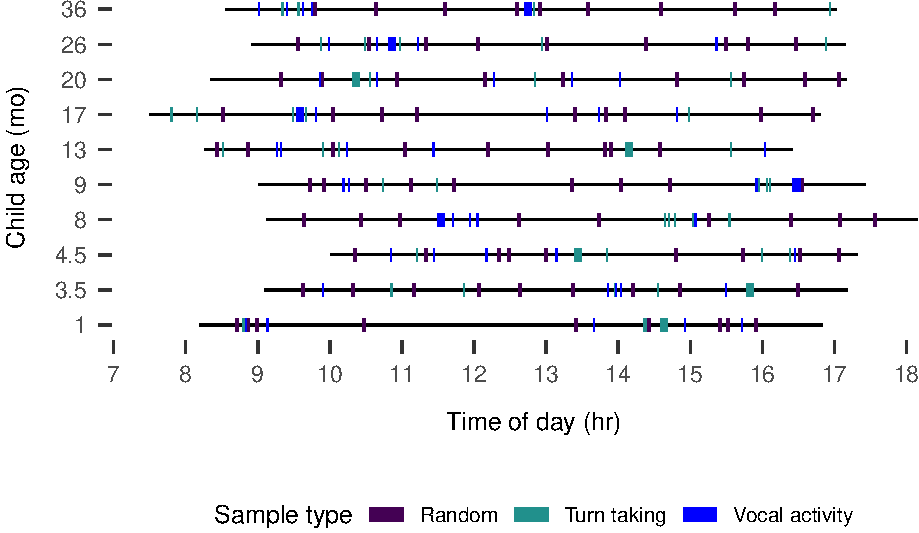
\includegraphics{Yeli-CLE_files/figure-latex/fig1-1.pdf}
\caption{\label{fig:fig1}Recording duration (black line) and sampled clips
(colored boxes) for each of the 10 recordings analyzed, sorted by child
age in months.}
\end{figure}

\subsection{Data selection and annotation}\label{methods-samples}

From the daylong recordings of 57 Rossel children, we selected 10
representative children between ages 0;0 and 3;0 for transcription and
analysis. The 10 children were selected to be spread between the target
age range (0;0--3;0) while also representing a range of typical maternal
education levels found in the community and being evenly split between
male and female children (\protect\hyperlink{tab1}{Table 1}). We
selected a series of non-overlapping sub-clips from each recording for
transcription (\protect\hyperlink{fig1}{Figure 1}) in the following
order: nine randomly-selected 2.5-minute clips, five manually-selected
\enquote{peak} turn-taking activity 1-minute clips, five
manually-selected \enquote{peak} \textbf{target child} vocal activity
1-minute clips, and one manually-selected 5-minute expansion of the best
one-minute clip, for a total of 37.5 minutes of transcribed audio for
each child (6.25 audio hours in total).

\textbf{Manual clip selection proceeded as follows: one person (the
first author or a non-Rossel research assistant) listened through the
entirety of each recording, documenting the approximate onset time,
duration, and notable features of any short period that they perceived
to be a \emph{burst} of turn taking and/or target-child vocalization;
judgments were made subjectively, and with reference to the lack of such
activity in other parts of the recording. After compiling a list
candidate bursts for each recording, the first author listened again to
each candidate, adding further notes about the diversity of target-child
vocalizations and the density of turn taking. Clips that overlapped with
previously transcribed segments or that featured significant background
noise were eliminated. From the remainder, the five 1-minute clips that
best demonstrated sequences of temporally contingent vocalization
between the target child and at least one other person were selected as
the \enquote{turn-taking} clips. From the remaining candidate clips, the
five that best demonstrated high density, high maturity, and high
diversity vocalizations by the target child were selected as the
\enquote{vocal activity} clips. After these ten 1-minute clips had been
transcribed for each recording (i.e., during the field visit), the first
author assessed each for its density of vocal and turn-taking activity
and searched for continuation of that activity before and after the
one-minute clip. The clip that best balanced dense, minimally
repetititious verbal activity with continuation in neighboring minutes
was selected to have a 5-minute extension window for further annotation.
All else being equal, we give preference to clips featuring speech from
underrepresented foreground speakers (e.g., adult males; see more
details at OMITTED-FOR-REVIEW).}

\textbf{We were limited to annotating these} sub-clips from only 10
children because of the time-intensive nature of transcribing these
naturalistic data; 1 minute of audio typically took approximately 60--70
minutes to be segmented into utterances, transcribed, annotated, and
loosely translated into English (\textasciitilde{}400 hours total). Yélî
Dnye is almost exclusively spoken on Rossel Island, where there is no
electricity (we use solar panels) and unreliable access to mobile data,
so transcription was completed over the course of three 4--6 week visits
to the island in 2016, 2018, and 2019.

We used the ACLEW Annotation Scheme (Casillas et al., 2017) in ELAN
(Wittenburg, Brugman, Russel, Klassmann, \& Sloetjes, 2006) to
transcribe and annotate all hearable speech in the clips. Using both the
audio and photo context, we segmented out the utterances and ascribed
them to individual speakers (e.g., older brother, mother, aunt, etc.).
We then annotated the vocal maturity of each utterance produced by the
target child (non-canonical babble/canonical babble/single
word/multi-word/unsure) and annotated the addressee of all speech from
other speakers (addressed to the target child/one or more other
children/one or more adults/a mix of adults and children/any
animal/other/unsure).

\textbf{Regarding vocal maturity annotations, an vocalization was
considered \enquote{single word} if it contained a single recognizable
(transcribed) lexical type (e.g., \enquote{mine}, \enquote{mine mine})
and \enquote{multi-word} if it contained more than one lexical type
(e.g., \enquote{my mango}), with non-lexical lingusitic vocalizations
annotated as \enquote{canonical babble} (containing at least one
consonant with an adult-like transition with its neighboring vocalic
sound(s)) or \enquote{non-canonical babble}, and non-linguistic
vocalizations classified as \enquote{crying} or \enquote{laughing}.
Vocalizations that were too ambiguous to make a decision were marked as
\enquote{unsure}. Vegetative sounds (e.g., sneezes) were ignored.}

**Regarding addressee annotations, the audio and photo context were used
to review who each speaker was talking to for each utterance; utterances
were only considered directed to the target child when the native
Rossel-speaking research assistant and first author felt certain of this
judgment given the context. Utterances were otherwise classified as
directed to a \enquote{child} (1+ children; a group of children
including the target child), \enquote{adult} (1+ adults), \enquote{both}
(1+ children and 1+ adults; a group that may include the target child),
\enquote{animal} (1+ animals), \enquote{other} (a clear addressee that
doesn't fit into the other categories), or \enquote{unsure} (not enough
evidence to make a judgment).

Note that all transcription** and annotation was done together by the
first author and one of three community members (all native Yélî Dnye
speakers). The community-based research assistants personally knew all
the families in the recordings, and were able to use their own
experience, the discourse context, and information from the accompanying
photos in reporting what was said and to whom speech was addressed for
each utterance. \textbf{These annotations relied on mutual agreement
between the first author and the Rossel research assistant, so there is
no direct way to estimate interrater reliability for the NN target-child
vocalizations and NN other-speaker vocalizations discovered in the
clips. That said, independent vocal maturity annotations of these same
target child vocalizations in a different studied revealed a highly
similar pattern of results (OMITTED-FOR-REVIEW).} Detailed manuals and
self-guided training materials, including a \enquote{gold standard test}
for this annotation scheme can be found at OMITTED-FOR-REVIEW.

In what follows we first analyze the nine randomly selected 2.5-minute
clips from each child to establish a baseline view of their speech
environment, focusing on the effects of child age, time of day,
household size, and number of speakers on the rate of target
child-directed (TCDS) and other-directed speech (ODS). Next, we repeat
these analyses, focusing instead only on the turn-taking clips to gain a
view of the speech environment as it appears during the peak
interactions for the day. Then as a first approximation of children's
linguistic development, we map a coarse trajectory of children's use of
babble, first words, and multi-word utterances. \textbf{Lastly, we
compare our findings to those from the Tseltal Mayan community, and
briefly relate our results to the larger literature on child-directed
speech and its role in language development.}

\subsection{Statistical models}\label{statistical-models}

We conducted all analyses in R, using the glmmTMB package to run
generalized linear mixed-effects regressions (M. E. Brooks et al., 2017;
R Core Team, 2019) and ggplot2 to generate figures (Wickham, 2016). This
dataset and analysis are available at URL\_MASKED\_FOR\_REVIEW. TCDS and
ODS minutes per hour are naturally restricted to non-negative
(0--infinity) values, causing the distributional variance of those
measures to become positively skewed. To address this issue we use
negative binomial regressions, which can better fit non-negative,
overdispersed data (M. E. Brooks et al., 2017; Smithson \& Merkle,
2013). There were also many cases of zero minutes of TCDS across the
clips---for example, this often occurred in the randomly sampled clips
when the child was sleeping in a quiet area. To handle this additional
distributional characteristic of the data, we added a zero-inflation
model to TCDS analysis which, in addition to the count model of TCDS
(e.g., testing effects of age on the input rate), creates a binary model
to evaluate the likelihood of TCDS being used at all. More conventional,
gaussian linear mixed-effects regressions with log-transformed dependent
variables are provided in the Supplementary Materials, but are
qualitatively similar to what we report here.

\section{Results}\label{results}

The models included the following predictors: child age (months;
centered and standardized), household size (number of people; centered
and standardized), number of non-target-child speakers present in that
clip (centered and standardized), and time of day at the start of the
clip (factor: \enquote{morning} = before 11:00; \enquote{midday} =
11:00--13:00; \enquote{afternoon} = after 13:00). We also included
two-way interactions of (a) child age and the number of speakers present
and (b) child age and time of day, with a random effect of child. For
the zero-inflation model of TCDS, we included the number of speakers
present. We limit our discussion to significant effects; full model
results are provided in the Supplementary Materials.

\begin{figure}
\centering
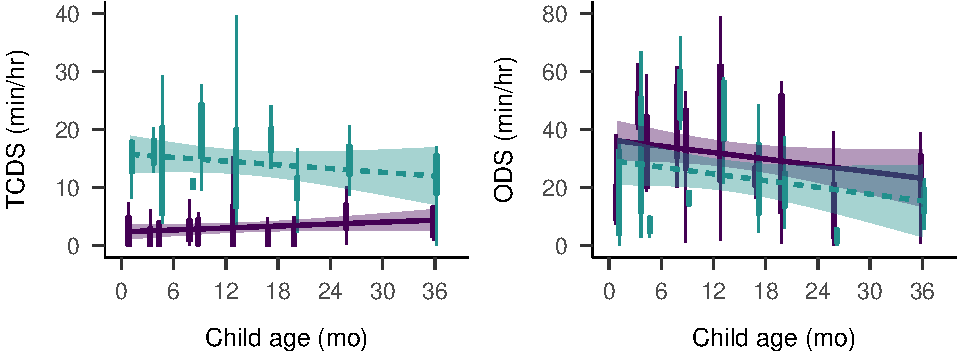
\includegraphics{Yeli-CLE_files/figure-latex/fig2-1.pdf}
\caption{\label{fig:fig2}Estimates of TCDS min/hr (left) and ODS min/hr
(right) across the sampled age range. Each box plot summarizes the data
for one child from the randomly sampled clips (purple; solid) or the
turn taking clips (green; dashed). Bands on the linear trends show 95\%
confidence intervals.}
\end{figure}

\subsection{Target-child-directed speech
(TCDS)}\label{target-child-directed-speech-tcds}

In the random sample, these 10 children heard an average of 3.13 minutes
of speech directly addressed to them per hour (median = 2.95; range =
1.58--6.26; \protect\hyperlink{fig2}{Figure 2} left panel, purple/solid
summaries). For comparison, this is slightly less than reported values
using a near-identical method of data collection, annotation, and
analysis in a Tseltal Mayan community (3.6 minutes per hour for children
under 3;0; Casillas et al. (2019)) and comparable to what has been
reported using a similar method in a Tsimane community (1.6--4.8 minutes
per hour for children under 3;0 depending on what speech is counted;
Scaff et al., in preparation).

The zero-inflated negative binomial regression of TCDS minutes per hour
(N = 90, log-likelihood = -195.26, overdispersion estimate = 3.37)
suggested significant effects of child age, time of day, and their
interaction on the rate at which children are directly addressed. First,
the older children heard a small but significantly greater amount of
TCDS per hour (\protect\hyperlink{fig2}{Figure 2} left panel
purple/solid summaries; B = 0.73, SD = 0.23, z = 3.20, p \textless{}
0.01). Overall, these children were also more likely to hear TCDS in the
mornings (\protect\hyperlink{fig3}{Figure 3} top left panel), with
significantly higher TCDS rates in the morning compared to both midday
(midday-vs-morning: B = 0.80, SD = 0.36, z = 2.23, p = 0.03) and the
afternoon (afternoon-vs-morning: B = 0.54, SD = 0.26, z = 2.10, p =
0.04), and no significant difference in TCDS rate between midday and the
afternoon. However, the time-of-day pattern changed with child age.
Older children were more likely than younger children to show a peak in
TCDS during midday, with a decrease in TCDS between midday and the
afternoon (midday-vs-afternoon: B = -0.60, SD = 0.29, z = -2.04, p =
0.04) and marginally less TCDS in the morning than at midday
(midday-vs-morning: B = -0.59, SD = 0.30, z = -1.94, p = 0.05). There
were no significant effects in either the count or the zero-inflation
models.

Children heard TCDS from a variety of different speakers. Most TCDS came
from adults (mean = 72.65\%, median = 75.51\%, range = 41.41--100\%). On
average, 82.35\% of the total TCDS minutes from adults came from women.
However, an increasing quantity of TCDS with age came from child
speakers (child-TCDS, e.g., from siblings, cousins, or neighbors;
C-TCDS); a Spearman's correlation showed a significant positive
relationship between the average proportion of C-TCDS in a clip and
target child age (Spearman's \emph{rho} = 0.78; \emph{p} = 0.01).

\begin{figure}
\centering
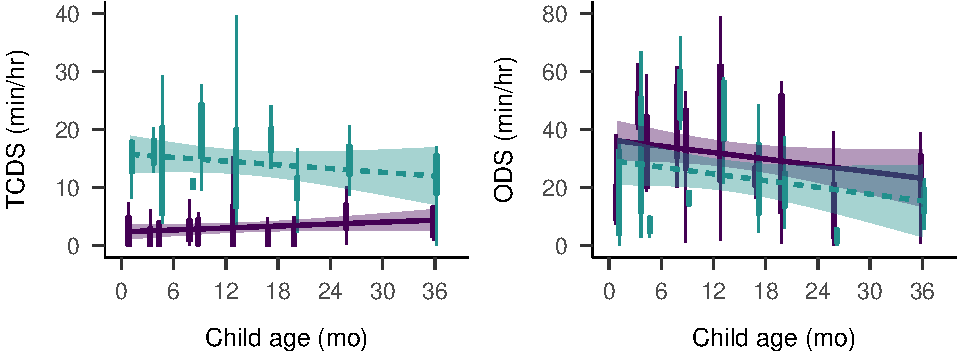
\includegraphics{Yeli-CLE_files/figure-latex/fig3-1.pdf}
\caption{\label{fig:fig3}Estimates of TCDS min/hr (left panels) and ODS
min/hr (right panels) across the recorded day in the random clips (top
panels) and turn-taking (bottom panels) clips. Each box plot summarizes
the data for children age 1;0 and younger (light) or age 1;0 and older
(dark) at the given time of day.}
\end{figure}

\subsection{Other-directed speech
(ODS)}\label{other-directed-speech-ods}

In the random sample, these children heard an average of 35.90 minutes
of other-directed speech per hour (\protect\hyperlink{fig2}{Figure 2}
right panel, purple/solid summaries; median = 32.37; range =
20.20--53.78): that is more than eleven times the average quantity of
speech directed to them, with many clips displaying near-continuous
background speech. For comparison, the prior estimate for Tseltal
children using near-parallel methods found an average of 21 minutes of
overhearable speech per hour (Casillas et al., 2019), and a recent study
of North American children's daylong recordings found that
adult-directed speech (a subset of ODS) occurred at a rate of 7.3
minutes per hour (Bergelson, Amatuni, Dailey, Koorathota, \& Tor,
2019a).

The negative binomial regression of other-directed speech rate (N = 90,
log-likelihood = -370.87, overdispersion estimate = 9.14) revealed
effects of child age, number of speakers present, and time of day on the
rate of ODS encountered. The rate of ODS significantly decreased with
child age (\protect\hyperlink{fig2}{Figure 2} right panel, purple/solid
summaries; B = -0.57, SD = 0.17, z = -3.28, p \textless{} 0.01) and
significantly increased in the presence of more speakers (B = 0.50, SD =
0.05, z = 10.07, p \textless{} 0.001). Across the randomly selected
clips, there were an average of 6.19 speakers present other than the
target child (median = 6; range = 1--19), an average of 59.99\% of whom
were adults. Comparing again to Tseltal and North American English, in
which the average number of speakers present, not including the target
child, was 3.44 and 3.9 respectively (Bergelson et al., 2019a; Casillas
et al., 2019), we can infer that the increased rate of ODS on Rossel
Island is due in part to there simply being more speakers present.
Time-of-day effects on ODS only came through in an interaction with
child age (\protect\hyperlink{fig3}{Figure 3} top right panel). In
particular, older children heard a pattern of ODS mirroring the general
pattern of TCDS; significantly more ODS in the mornings compared to
midday (midday-vs-morning: B = 0.65, SD = 0.20, z = 3.23, p \textless{}
0.01) and the afternoon (afternoon-vs-morning: B = 0.37, SD = 0.15, z =
2.50, p = 0.01). There were no other significant effects on ODS rate.

In sum, the random baseline rates of TCDS and ODS in children's speech
environments are influenced by child age (TCDS increases, ODS
decreases), time of day (both generally peak in the morning), and their
interaction (older children hear more TCDS and less ODS than younger
children at midday). The rate of ODS is also impacted by the number of
speakers present. Correlational results suggest that TCDS comes
increasingly from other children over the first three years. That said,
the baseline rate of TCDS is low, on par with estimates in other
small-scale rural communities (Casillas et al., 2019; Scaff et al., in
preparation), while the ODS rate is quite high relative to estimates in
prior work.

\subsection{TCDS and ODS during interactional
peaks}\label{tcds-and-ods-during-interactional-peaks}

If we instead investigate the rates of TCDS and ODS encountered by these
children during interactional peaks, a different picture emerges
(\protect\hyperlink{fig2}{Figures 2} and \protect\hyperlink{fig3}{3}
green/dashed summaries). The children heard much more TCDS in the
turn-taking clips---14.45 min/hr; more than four times the rate of TCDS
in the random baseline (\protect\hyperlink{fig2}{Figure 2}, left panel,
green/dashed summaries; median = 15.07; range = 9.61--18.73). Children
also heard a reduced rate of ODS: 25.27 min/hr (70.39\% of the
random-sample ODS rate, \protect\hyperlink{fig2}{Figure 2}, right panel,
green/dashed summaries; median = 19.59; range = 6.68--60.18).

The negative binomial mixed-effects regression of TCDS (N = 55,
log-likelihood = -183.25, overdispersion estimate = 2.91) revealed a
significant decrease with child age (B = -0.63, SD = 0.27, z = -2.33, p
= 0.02) and a significant interaction between child age and time of day;
TCDS rate during interactional peaks was marginally higher for older
children at morning compared to midday (midday-vs-morning: B = 0.53, SD
= 0.28, z = 1.89, p = 0.06) and significantly higher in the afternoon
than at midday (midday-vs-afternoon: B = 0.61, SD = 0.28, z = 2.17, p =
0.03; see \protect\hyperlink{fig3}{Figure 3}, bottom left panel).

As in the random sample, an increasing portion of TCDS during
interactional peaks came from other children with age. While, overall,
more of the TCDS in interactional peaks came from adults than in the
random clips (mean = 82.68\%, median = 88.04\%, range = 50--100\%), a
Spearman's correlation showed an even stronger positive relationship
between the average proportion of child TCDS in a clip and target child
age (Spearman's \emph{rho} = 0.92; \emph{p} = \textless{} 0.001).
Notably, women contributed proportionally less TCDS during interactional
peaks than they did during the random clips: on average, women
contributed 61.55\% of the children's TCDS minutes from adults in the
turn-taking clips (compared to 82.35\% in the random clips). In brief,
compared to the random sample, interactional peaks included more
directed speech from men and, for older target children, more directed
speech from other children.

The negative binomial mixed-effects regression of ODS (N = 55,
log-likelihood = -202.60, overdispersion estimate = 4.66) only revealed
a significant effect of number of speakers. As before, ODS rates were
higher when more speakers were present (B = 0.56, SD = 0.08, z = 6.76, p
\textless{} 0.001). There were no other significant effects on ODS rate
(\protect\hyperlink{fig3}{Figure 3}, bottom right panel).

Overall, the results suggest that these children typically hear very
little directly addressed speech, but that interactional peaks provide
opportunities for dense input. While the majority of directed speech
comes from women, an increasing portion of it comes from other children
with age, and directed speech from men is more likely during
interactional peaks. Directed and overhearable speech are most likely to
occur during the morning, before most of the household has dispersed for
their work activities, similar to other findings from subsistence
farming households (Casillas et al., 2019). However, older children are
more likely than younger children to show higher input rates at midday,
perhaps due to their increased interactions with other children while
adults attend to gardening and domestic tasks. Possibly because of the
large number of speakers present, these children were also in the
vicinity of voluminous overhearable speech, underscoring the
availability of other-addressed speech as a resource for linguistic
input in this context.

\subsection{Vocal maturity}\label{vocal-maturity}

Given the low baseline rate of directed speech, one might expect that
Rossel children's early linguistic development, particularly the onset
and use of single- and multi-word utterances, shows delays in comparison
to children growing up in more CDS-rich environments. We plotted the
proportion of all linguistic vocalizations for each child (i.e.,
discarding laughter, crying, or unknown-types; leaving a total of 4308
vocalizations) that fell into the following categories: non-canonical
babble, canonical babble, single-word utterance, or multi-word
utterance. Children are expected to traverse all four types of
vocalization during development such that they primarily produce single-
and multi-word utterances by age three.

In the onset of use for canonical babble, first words, and multi-word
utterances, these Rossel children's vocalization data closely resemble
expectations based on populations of children who hear more CDS
(\protect\hyperlink{fig4}{Figure 4}). Canonical babble appears in the
second half of the first year, first words appear around the first
birthday, and multi-word utterances appear a few months after that
(Frank et al., in preparation; P. K. Kuhl, 2004; Pine \& Lieven, 1993;
Slobin, 1970; Tomasello \& Brooks, 1999; Warlaumont, Richards,
Gilkerson, \& Oller, 2014). Rossel children also far exceeded the
canonical babbling ratio (CBR) associated with major developmental delay
(proportional use of speech-like vocalizations \textgreater{} 0.15 by
0;10; Cychosz et al., under review; Oller, Eilers, Basinger, Steffens,
\& Urbano, 1995); the minimum CBR among Rossel children 0;9 and older
was 0.22 (mean = 0.63; median = 0.68; range = 0.22--0.86).

Over all annotated clips, children produced an average of 7.18
linguistic vocalizations per minute (median = 7.79; range = 4.57--8.95),
less frequently than children in short recordings of American
infant-caregiver interaction (Oller et al., 1995) but similar to
estimates for Tseltal children (Brown, 2011; Casillas et al., 2019).

\begin{figure}
\centering
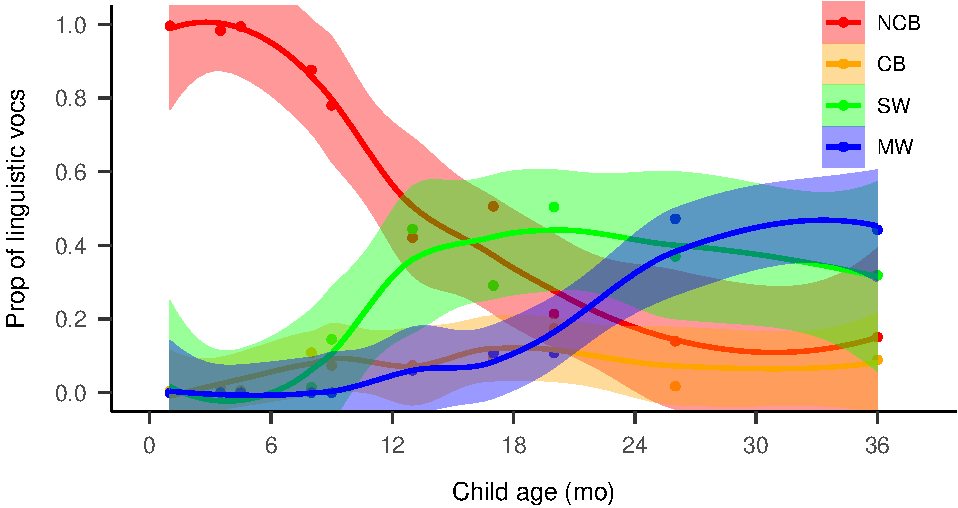
\includegraphics{Yeli-CLE_files/figure-latex/fig4-1.pdf}
\caption{\label{fig:fig4}Proportion of vocalization types used by children
across age (NCB = Non-canonical babble, CB = Canonical babble, SW =
single word utterance, MW = multi-word utterance).}
\end{figure}

\section{Discussion}\label{disc}

We analyzed the speech environments of 10 Rossel children under age 3;0
to investigate: (a) how often children were spoken to directly, (b) how
much other overhearable speech is available to them, and (c) how these
sources of linguistic input are shaped by child age and interactional
context. \textbf{We then additionally conducted a preliminary
investigation into} (d) whether this (relatively) low rate of directed
input appears to impact their early production milestones.

\textbf{By investigating the language environments of children in this
child-centric subsistence farming context, we aimed to provide a new and
critical comparative datapoint to a research area that has previously
confounded differences in child-directed speech ideology with
differences in broad lifestyle features (post-industrial/nuclear
vs.~subsistence-farming/multi-generational; Casillas et al. (2019),
Shneidman \& Goldin-Meadow (2012)). Our idea was that, if Rossel
children's language environments pattern like North American ones, it
would support that idea that caregiver ideology drives substantial
differences in language input, whereas if they patterned like Tseltal
environments, it would instead support the idea that lifestyle drives
substantial differences. Overall, our findings point toward broad
effects of lifestyle on the quantity of directed and overheard speech
children hear. Evidence for the influence of CDS ideologies only begins
to emerge when we look at patterns in \emph{who} speaks to the target
child, not at overall rates of linguistic input.}

\subsection{\texorpdfstring{\textbf{Input rate similarities across
subsistence farming
communities}}{Input rate similarities across subsistence farming communities}}\label{input-rate-similarities-across-subsistence-farming-communities}

Based on prior ethnographic work, we \textbf{hypothesized} that
\textbf{Rossel} children would hear frequent child-directed speech
(Brown \& Casillas, in press). In fact, \textbf{Rossel} children were
rarely directly addressed \textbf{over the course of the day. We found a
baseline rate of TCDS} comparable to that found in a Tseltal community
where \textbf{infrequent use of} TCDS is one means to socializing
children into attending to their surroundings \textbf{(Rossel: 3.13 TCDS
min/hr vs.~Tseltal: 3.63). As in the case of Tseltal children, this
relatively low rate of TCDS was not associated with any delay in the
appearance of vocal maturity milestones, including the use of single and
multi-word utterances. Since we know from prior, in-depth ethnographic
work that caregivers' ideas about talking to young children do, in fact,
differ enormously in these two communities (Brown, 2011, 2014; Brown \&
Casillas, in press), we attribute the similarity in baseline rates of
TCDS to the fact that all these children are growing up in
multi-generational, subsistence farming households. This inference is
bolstered by the fact that fluctuations in TCDS rate over the day in the
Rossel Island data are highly similar to those reported for
Tseltal---peak rates in the morning, with older children eliciting more
TCDS during midday hours than younger children (Casillas et al., 2019),
and with ODS rate following a similar contour. While a basic
afternoon-dip pattern has been shown in at least one set of North
American home recordings (Greenwood et al., 2011; Soderstrom \&
Wittebolle, 2013), the activities and total number of speakers present
during periods of peak linguistic input periods are likely to be
different across these economic contexts; an important avenue for future
research. In line with prior work linking high caregiver workload to
less CDS, our prediction is that the Tseltal and Rossel Island
fluctuations derive from (broadly) similar tasks associated with their
subsistence farming lifesyles (see also Kaluli, Samoan, Gusii, and
Yucatec; R. A. LeVine et al. (1996); Ochs (1988); Schieffelin (1990);
see Gaskins (2006) for a review).}

\textbf{We had hypothesized that cultural differences in quantity of
caregiver talk to children would be most visible in the turn-taking
clips, which are selected in particular for their insight into caregiver
responsiveness patterns. Against expectations, we found a similar
overall rate of TCDS in the Rossel Island data compared to that of the
Tseltal children (Rossel: 14.45 TCDS min/hr vs.~Tseltal: 13.28). In both
cultural contexts, peak TCDS clips displayed around four times the
directed speech rate as the baseline, though we note that this relative
increase was greater in the case of the Rossel data than the Tseltal
data (Rossel: 4.62x the random rate vs.~Tseltal: 3.66x).}

\subsection{\texorpdfstring{\textbf{Input source differences across
subsistence farming
communities}}{Input source differences across subsistence farming communities}}\label{input-source-differences-across-subsistence-farming-communities}

\textbf{One distinctive feature of the Rossel Island data that was not
oberved for Tseltal is the division of TCDS among women, men, and other
children. On Rossel Island, it is common for both adult and child,
females and males, to attend to the care of young children (Brown \&
Casillas, in press). In line with these observations, we find that
Rossel children hear more CDS from other children than Tseltal children
do (Rossel: 27\% of TCDS vs.~Tseltal 20\%), and that the proportion of
TCDS from other children increases with age, a pattern not found for
Tseltal children in this age range (Casillas et al., 2019).
Additionally, TCDS from men was far more frequent in the Rossel Island
data, making up nearly 20\% of adult TCDS in the random baseline and
nearly 40\% of adult TCDS in the turn-taking clips.\footnote{For
  comparison, men's TCDS was absent in 4 out of 10 Tseltal children's
  samples and was outpaced 12-to-1 or more by TCDS from women in the
  other 6 children's samples.} We take this substantial proportion of
TCDS from children and men as evidence that caregiving is indeed divided
among many types of speakers in Rossel communities (Brown \& Casillas,
in press); note that, together, child and adult male speakers contribute
more than half of the TCDS during interactional peaks. In brief, we only
get a glimpse into the different caregiving arrangements between the
Tseltal and Rossel cultural contexts with respect to who is talking to
the target child, and not with respec to how often the child is being
talked to.}

\textbf{The} increase in TCDS from other children recalls findings from
Shneidman and Goldin-Meadow (Shneidman \& Goldin-Meadow (2012); see also
(Brown, 2011; Brown \& Casillas, in press)) in which Yucatec Mayan
children's directed speech rate increased enormously between ages one
and three\textbf{---much more than the increase observed in these Rossel
children's recordings---}primarily due to increased input from other
children\textbf{.} Interestingly, \textbf{data from the Tseltal}
community---culturally more proximal to the Yucatec families studied in
Shneidman and Goldin-Meadow (2012)---\textbf{show} no evidence for
increased input from other children in this same age range (0;0--3;0;
Casillas et al., 2019)\textbf{, possibly because Tseltal children only
begin} to \textbf{more fully} engage in independent, extended play with
other children \emph{after} age three. In \textbf{contrast,}
independence \textbf{has been documented as} a primary concern for
parents of young children \textbf{on Rossel Island}; from early
toddlerhood Rossel children are encouraged to choose how they dress,
when and what to eat, and whom to visit (Brown \& Casillas, in press).
The formation of hamlets in a cluster around a shared open area, often
close to a shallow swimming area, further nurtures a sense of safe, free
space in which children can wander. These features of childhood on
Rossel Island support extended independent play with other children from
an early age and may help explain the strongly increasing presence of
child TCDS in the present data. Further work combining the
\textbf{time-of-day and interactant} effects found here with
ethnographic interview data are needed to explore these ideas in
full\textbf{.}

\subsection{\texorpdfstring{\textbf{Replicating daylong language
environment
patterns}}{Replicating daylong language environment patterns}}\label{replicating-daylong-language-environment-patterns}

\textbf{Prior work using daylong audio recordings in both Western and
non-Western contexts} led us to expect that the quantity of TCDS would
be \textbf{relatively stable} across the age range studied\textbf{, that
ODS rate would decrease with age, and that TCDS would be non-uniformly
distributed over the recording day (Abney et al., 2017; Bergelson et
al., 2019b; Casillas et al., 2019; Scaff et al., in preparation).
}Counter to expectations, we found a small but significant increase in
TCDS rate with child age in the random clips and a small and significant
\emph{decrease} in TCDS rate with age in the turn-taking clips. The
age-related baseline increase in TCDS may derive from more frequent
participation in independent play with other children; in prior work,
increased proportional input from other children was also associated
with an increase in overall input rate (Shneidman \& Goldin-Meadow,
2012). The age-related decrease in TCDS rate during peak interactional
moments was not expected, but may \textbf{also} be attributable to this
change in interactional partners with age; if adults are more likely to
be the source of TCDS during interactional peaks for younger children,
they may also provide more voluminous speech during those peaks than
other children do during interactional peaks later in development. Sleep
during the day may also help explain these patterns; if older children
sleep less than younger children, they may be more likely hear more TCDS
during random but not peak-based clips. All of these explanations
require follow-up work from a larger sample of children and, ideally,
from a larger sample of their interactions throughout the day.
\textbf{Finally, consistent with prior daylong language environment
analyses,} ODS rate decreased with age\textbf{, and the random and
turn-taking clips across the day revealed substantial fluctuations in
TCDS rate (Abney et al., 2017; Bergelson et al., 2019b; Casillas et al.,
2019; Scaff et al., in preparation).}

\textbf{One implication of our findings is that TCDS rate estimates from
daylong data do not appear to be} effective at distinguishing distinct
caregiver attitudes toward talking to young children. While Rossel
caregivers view their children, even their young infants, as potential
co-interactants in conversational play (Brown \& Casillas, in press),
the circumstances of everyday life shape the broader linguistic
landscape such that most of what children hear is talk between others.
We suggest that, in the daylong context, caregivers from these two
subsistence farming communities are preoccupied for most of the day with
social and domestic commitments in which they are motivated to converse
with the other adults and (older) children present; not just to get
their daily tasks done but also because these more mature speakers
enable more complex verbal interactions and social routines\textbf{.
Rather,} we suspect that caregiver attitudes about how to engage
children in interaction are \textbf{more} clearly expressed
\textbf{during interactional peaks and, even then, primarily via
behaviors more nuanced than input quantity. In the case of Rossel
Island, we saw }not only more TCDS but also TCDS from more diverse
speaker types** during interactional peaks. We suggest, then, that** the
forces shaping the rate of Rossel children's linguistic input are
somewhat different from the forces shaping the content and sources of
their linguistic input. \textbf{In order to comparatively examine
culturally distinct codes of verbal interaction in children's at-home
speech environments, future work should focus not only the rate, but
also the sources and content, of the speech children are exposed to,
perhaps using strategic subsampling similar to what was implemented in
the present study.}

\subsection{\texorpdfstring{\textbf{Implications for theories of
language
learning}}{Implications for theories of language learning}}\label{implications-for-theories-of-language-learning}

\textbf{Despite hearing relatively little directed linguistic input,
these 10 Rossel children show no sign of delay in their achievement of
early linguistic milestones, including the use of single and multi-word
utterances. This finding is hard to explain under any theory of language
learning that requires substantial linguistic input (see also Casillas
et al., 2019). While prior evidence predicts a highly robust onset of
canonical babble ({\textbf{???}}; but see also Lee, Jhang, Relyea, Chen,
\& Oller, 2018; Oller et al., 1995; e.g., Oller, Eilers, Neal, \&
Cobo-Lewis, 1998), the stable use of individual phonological segments in
speech-like babble and the subsequent appearance of recognizable words
is indeed variable between children (see also McCune \& Vihman, 2001;
McGillion et al., 2017) and, further on, children's early productive
vocabulary size predicts their later syntactic development, including
early word combinations (Frank et al., in preparation; Marchman et al.,
2004). In sum, while a stable onset for canonical babble is expected
cross-linguistically, there is no such expectation for the onset of
lexical and multi-word utterances.}

\textbf{Following a similar set of findings regarding both the language
environment and vocal maturity of Tseltal-learning children, Casillas
and colleagues (2019) suggested three ways in which children might
proceed in language learning without delay despite hearing relatively
little directed speech: (a) an ability to learn from observing others'
language use (see also de León, 2011; Rogoff et al., 2003; Shneidman,
2010; Shneidman \& Goldin-Meadow, 2012), (b) capitalizing on
regularities in language used during day-to-day routines, and (c)
benefiting from a natural cycle in which children frequently sleep
following short bursts of interactional linguistic input. In this third
case, the idea is that short-term memories of directed input are
consolidated before significant interference takes place (Gómez,
Bootzin, \& Nadel, 2006; Horváth, Liu, \& Plunkett, 2016; Kurdziel,
Duclos, \& Spencer, 2013; Mullally \& Maguire, 2014). These three
proposals, which are not mutually exclusive, may also apply in the case
of Rossel children, considering that the overall characteristics of the
environment are quite similar.}

\textbf{Mechanisms for language learning that efficiently capitalize on
sparse bursts of CDS and/or overhearable speech (e.g., massed learning,
as in Schwab \& Lew-Williams (2016); or attention to others' talk, as in
Akhtar (2005); Shneidman, Arroyo, Levine, \& Goldin-Meadow (2012)) are
supported by the current findings. Further, theoretical models of
language learning that: (a) make the most of each linguistic
\enquote{datapoint} in the input and (b) enable rapid uptake of streams
of talk (e.g., when observing speech between others) may be key to
explaining language development in this context. For example,
prediction-based models allow the learner to compare the predicted
vs.~observed properties of each utterance as it unfolds, with
recalibration when errors are detected (Chang, Dell, \& Bock, 2006;
Christiansen \& Chater, 2016; Elman, 1990, 1993; McCauley \&
Christiansen, 2017). Such models hypothetically make the most of each
utterance by rapidly updating knowledge on the basis of both the
occurrence and non-occurrence of expected events {[}see Rabagliati et
al. for a balanced overview{]}. In contrast, models of learning that
rely on pedagogical cueing or frequent and fitted responses to infant
vocalizations by an adult caregiver are not easily reconciled with the
results presented here, nor indeed those reported for several other
rural, traditional communities (Brown, 2014; Cristia, Dupoux, Gurven, \&
Stieglitz, 2017; Gaskins, 2006; Ochs \& Schieffelin, 1984; Scaff et al.,
in preparation; Shneidman \& Goldin-Meadow, 2012; Vogt, Mastin, \&
Schots, 2015).}

\subsection{\texorpdfstring{\textbf{Limitations}}{Limitations}}\label{limitations}

\textbf{Prior work establishing input-related variation in language
development has often focused on the relationship between child
vocabulary and input \enquote{quality} (e.g., Cartmill et al., 2013;
Hirsh-Pasek et al., 2015; Ramírez, Lytle, \& Kuhl, 2020;
Ramírez-Esparza, García-Sierra, \& Kuhl, 2014; Rowe, 2012), neither of
which we measure here. Vocabulary development on Rossel Island may
indeed be responsive to the type and quantity of CDS children
encounter---for example, referentially transparent utterances would
theoretically still facilitate the acquisition of word meanings. That
said, our impression is that such variation does not play a meaningful
role in Rossel children's development as a full-fledged members of the
language community. So, future work along those lines would likely be
limited to interpreting such effects with respect to the mechanisms
underlying lexical category formation, and not as prerequisites for
normative language development. With respect to input \enquote{quality}
we are similarly unable to assume that the features of language
experience considered to be \enquote{quality} in a US middle-class
context also happen to promote the suite of language behaviors
particular to Yélî Dnye speakers. Instead, we here use
target-child-directed speech as a proxy for the quantity of
\enquote{tailored} input children hear; that is, the quantity of input
known to be tailored for the child's attention and ability at the moment
the speech was uttered.}

\subsection{Conclusion}\label{disc-conclusion}

We estimate that, on average, children on Rossel Island under age 3;0
hear 3.13 minutes of directed speech per hour, with an average of 14.45
minutes per hour during peak interactive moments during the day. Most
directed speech comes from adults, but older children hear more directed
speech from other children. There is also an average 35.90 minutes per
hour of overhearable speech present. Older children heard more directed
speech and less overhearable speech than younger children. Bursts of
speech featuring mostly TCDS appear to be present from infancy onward.
Despite this relatively low rate of directed speech, these children's
vocal maturity appears on-track with norms for typically developing
children in many other populations (Cychosz et al., under review; Lee et
al., 2018; Warlaumont et al., 2014).

Our findings diverged in several ways from expectations developed on the
basis of prior ethnographic work in this community, including the
frequency of child-directed talk and the distribution of talk over the
course of the day. When considered together with data from a Tseltal
Mayan community, the findings suggest that \textbf{estimates of input
rate derived from daylong data are} far more sensitive to
\textbf{situational} variation (e.g., the number of speakers present)
than \textbf{they are} to established ideological variation in how
caregivers talk to children\textbf{.} Whether child language development
is better predicted by meaningful individual differences in average
\textbf{situational} variation \textbf{in input rate},
ideologically-based variation \textbf{in other verbal behaviors} (e.g.,
\textbf{who talks to the child}), or something inbetween is a question
for future work. Cross-cultural and cross-linguistic data will have a
major role to play in teasing out the causal factors at play in this
larger issue relating children's early linguistic experience to their
later language development.

Importantly, the data presented here come from an evolving corpus of
Yélî Dnye developmental data; any reader interested in citing
descriptive features of the Rossel child language environment is
strongly encouraged to visit the following address for up-to-date
estimates: URL\_MASKED\_FOR\_REVIEW. The information on that linked page
will include any new data, annotations, and analyses added after the
publication of this study.

\section{Acknowledgements}\label{acknowledgements}

\newpage

\section{References}\label{refs}

\begingroup
\setlength{\parindent}{-0.5in} \setlength{\leftskip}{0.5in}

\hypertarget{refs}{}
\hypertarget{ref-abney2017time}{}
Abney, D. H., Smith, L. B., \& Yu, C. (2017). It's time: Quantifying the
relevant time scales for joint attention. In G. Gunzelmann, A. Howes, T.
Tenbrink, \& E. Davelaar (Eds.), \emph{Proceedings of the 39th Annual
Meeting of the Cognitive Science Society} (pp. 1489--1494). London, UK.

\hypertarget{ref-akhtar2005robustness}{}
Akhtar, N. (2005). The robustness of learning through overhearing.
\emph{Developmental Science}, \emph{8}(2), 199--209.

\hypertarget{ref-bates1997inseparability}{}
Bates, E., \& Goodman, J. C. (1997). On the inseparability of grammar
and the lexicon: Evidence from acquisition, aphasia, and real-time
processing. \emph{Language and Cognitive Processes}, \emph{12}(5--6),
507--584.
doi:\href{https://doi.org/10.1080/016909697386628}{10.1080/016909697386628}

\hypertarget{ref-bergelsonIPbsl}{}
Bergelson, E., Alphen, P. van, Benneti, L., Bunce, J., Casillas, M.,
Guez, A., \ldots{} Cristia, A. (in preparation). Child language
environments in \textgreater{}2500 daylong recordings across 5
continents.

\hypertarget{ref-bergelson2019day}{}
Bergelson, E., Amatuni, A., Dailey, S., Koorathota, S., \& Tor, S.
(2019a). Day by day, hour by hour: Naturalistic language input to
infants. \emph{Developmental Science}, \emph{22}(1), e12715.
doi:\href{https://doi.org/10.1111/desc.12715}{10.1111/desc.12715}

\hypertarget{ref-bergelsoncasillas2019what}{}
Bergelson, E., Casillas, M., Soderstrom, M., Seidl, A., Warlaumont, A.
S., \& Amatuni, A. (2019b). What do North American babies hear? A
large-scale cross-corpus analysis. \emph{Developmental Science},
\emph{22}(1), e12724.
doi:\href{https://doi.org/10.1111/desc.12724}{10.1111/desc.12724}

\hypertarget{ref-brinchmann2019direct}{}
Brinchmann, E. I., Braeken, J., \& Lyster, S.-A. H. (2019). Is there a
direct relation between the development of vocabulary and grammar?
\emph{Developmental Science}, \emph{22}(1), e12709.
doi:\href{https://doi.org/10.1111/desc.12709}{10.1111/desc.12709}

\hypertarget{ref-brooks2017modeling}{}
Brooks, M. E., Kristensen, K., van Benthem, K. J., Magnusson, A., Berg,
C. W., Nielsen, A., \ldots{} Bolker, B. M. (2017). Modeling
zero-inflated count data with glmmTMB. \emph{bioRxiv}.
doi:\href{https://doi.org/10.1101/132753}{10.1101/132753}

\hypertarget{ref-brown2011cultural}{}
Brown, P. (2011). The cultural organization of attention. In A. Duranti,
E. Ochs, \& and Bambi B Schieffelin (Eds.), \emph{Handbook of Language
Socialization} (pp. 29--55). Malden, MA: Wiley-Blackwell.

\hypertarget{ref-brown2014interactional}{}
Brown, P. (2014). The interactional context of language learning in
Tzeltal. In I. Arnon, M. Casillas, C. Kurumada, \& B. Estigarribia
(Eds.), \emph{Language in interaction: Studies in honor of Eve V. Clark}
(pp. 51--82). Amsterdam, NL: John Benjamins.

\hypertarget{ref-brownIPchildrearing}{}
Brown, P., \& Casillas, M. (in press). Childrearing through social
interaction on Rossel Island, PNG. In A. J. Fentiman \& M. Goody (Eds.),
\emph{Esther Goody revisited: Exploring the legacy of an original
inter-disciplinarian} (pp. XX--XX). New York, NY: Berghahn.

\hypertarget{ref-brown2014language}{}
Brown, P., \& Gaskins, S. (2014). Language acquisition and language
socialization. In N. J. Enfield, P. Kockelman, \& J. Sidnell (Eds.),
\emph{Handbook of Linguistic Anthropology} (pp. 187--226). Cambridge,
UK: Cambridge University Press.
doi:\href{https://doi.org/10.1017/CBO9781139342872.010}{10.1017/CBO9781139342872.010}

\hypertarget{ref-cartmill2013quality}{}
Cartmill, E. A., Armstrong, B. F., Gleitman, L. R., Goldin-Meadow, S.,
Medina, T. N., \& Trueswell, J. C. (2013). Quality of early parent input
predicts child vocabulary 3 years later. \emph{Proceedings of the
National Academy of Sciences}, \emph{110}(28), 11278--11283.
doi:\href{https://doi.org/10.1073/pnas.1309518110}{10.1073/pnas.1309518110}

\hypertarget{ref-casillas2019stepbystep}{}
Casillas, M., \& Cristia, A. (2019). A step-by-step guide to collecting
and analyzing long-format speech environment (lfse) recordings.
\emph{Collabra: Psychology}, \emph{5}(1), 24.
doi:\href{https://doi.org/10.1525/collabra.209}{10.1525/collabra.209}

\hypertarget{ref-casillas2019early}{}
Casillas, M., Brown, P., \& Levinson, S. C. (2019). Early language
experience in a {[}tseltal mayan{]} village. \emph{Child Development},
\emph{OnlineOpen}(X), XX--XX.

\hypertarget{ref-casillas2017ACLEWDAS}{}
Casillas, M., Bunce, J., Soderstrom, M., Rosemberg, C., Migdalek, M.,
Alam, F., \ldots{} Garrison, H. (2017). Introduction: The ACLEW DAS
template {[}training materials{]}. Retrieved from
\url{https://osf.io/aknjv/}

\hypertarget{ref-chang2006becoming}{}
Chang, F., Dell, G. S., \& Bock, K. (2006). Becoming syntactic.
\emph{Psychological Review}, \emph{113}(2), 234.

\hypertarget{ref-christiansen2016now}{}
Christiansen, M. H., \& Chater, N. (2016). The now-or-never bottleneck:
A fundamental constraint on language. \emph{Behavioral and Brain
Sciences}, \emph{39}.

\hypertarget{ref-cristia2017child}{}
Cristia, A., Dupoux, E., Gurven, M., \& Stieglitz, J. (2017).
Child-directed speech is infrequent in a forager-farmer population: A
time allocation study. \emph{Child Development}, \emph{Early View},
1--15. doi:\href{https://doi.org/10.1111/cdev.12974}{10.1111/cdev.12974}

\hypertarget{ref-cychoszURcanonical}{}
Cychosz, M., Cristia, A., Bergelson, E., Casillas, M., Baudet, G.,
Warlaumont, A. S., \ldots{} Seidl, A. (under review). Canonical babble
development in a large-scale crosslinguistic corpus. Retrieved from
\url{https://osf.io/ca6qu/}

\hypertarget{ref-deleon2011language}{}
de León, L. (2011). Language socialization and multiparty participation
frameworks. In A. Duranti, E. Ochs, \& and Bambi B Schieffelin (Eds.),
\emph{Handbook of Language Socialization} (pp. 81--111). Malden, MA:
Wiley-Blackwell.
doi:\href{https://doi.org/10.1002/9781444342901.ch4}{10.1002/9781444342901.ch4}

\hypertarget{ref-elman1990finding}{}
Elman, J. L. (1990). Finding structure in time. \emph{Cognitive
Science}, \emph{14}(2), 179--211.

\hypertarget{ref-elman1993learning}{}
Elman, J. L. (1993). Learning and development in neural networks: The
importance of starting small. \emph{Cognition}, \emph{48}(1), 71--99.

\hypertarget{ref-frankIPvariability}{}
Frank, M. C., Braginsky, M., Marchman, V. A., \& Yurovsky, D. (in
preparation). \emph{Variability and consistency in early language
learning: The Wordbank project}. Retrieved from
\url{https://langcog.github.io/wordbank-book/}

\hypertarget{ref-gaskins2000childrens}{}
Gaskins, S. (2000). Children's daily activities in a Mayan village: A
culturally grounded description. \emph{Cross-Cultural Research},
\emph{34}(4), 375--389.
doi:\href{https://doi.org/10.1177/106939710003400405}{10.1177/106939710003400405}

\hypertarget{ref-gaskins2006cultural}{}
Gaskins, S. (2006). Cultural perspectives on infant--caregiver
interaction. In N. J. Enfield \& S. Levinson (Eds.), \emph{Roots of
Human Sociality: Culture, Cognition and Interaction} (pp. 279--298).
Oxford: Berg.

\hypertarget{ref-gomez2006naps}{}
Gómez, R. L., Bootzin, R. R., \& Nadel, L. (2006). Naps promote
abstraction in language-learning infants. \emph{Psychological Science},
\emph{17}(8), 670--674.
doi:\href{https://doi.org/10.1111/j.1467-9280.2006.01764.x}{10.1111/j.1467-9280.2006.01764.x}

\hypertarget{ref-greenwood2011assessing}{}
Greenwood, C. R., Thiemann-Bourque, K., Walker, D., Buzhardt, J., \&
Gilkerson, J. (2011). Assessing children's home language environments
using automatic speech recognition technology. \emph{Communication
Disorders Quarterly}, \emph{32}(2), 83--92.
doi:\href{https://doi.org/10.1177/1525740110367826}{10.1177/1525740110367826}

\hypertarget{ref-hart1995meaningful}{}
Hart, B., \& Risley, T. R. (1995). \emph{Meaningful Differences in the
Everyday Experience of Young American Children}. Paul H. Brookes
Publishing.

\hypertarget{ref-hirshpasek2015contribution}{}
Hirsh-Pasek, K., Adamson, L. B., Bakeman, R., Owen, M. T., Golinkoff, R.
M., Pace, A., \ldots{} Suma, K. (2015). The contribution of early
communication quality to low-income children's language success.
\emph{Psychological Science}, \emph{26}(7), 1071--1083.
doi:\href{https://doi.org/10.1177/0956797615581493}{10.1177/0956797615581493}

\hypertarget{ref-hoff2003specificity}{}
Hoff, E. (2003). The specificity of environmental influence:
Socioeconomic status affects early vocabulary development via maternal
speech. \emph{Child Development}, \emph{74}(5), 1368--1378.
doi:\href{https://doi.org/10.3389/fpsyg.2015.01492}{10.3389/fpsyg.2015.01492}

\hypertarget{ref-horvath2016daytime}{}
Horváth, K., Liu, S., \& Plunkett, K. (2016). A daytime nap facilitates
generalization of word meanings in young toddlers. \emph{Sleep},
\emph{39}(1), 203--207.
doi:\href{https://doi.org/10.5665/sleep.5348}{10.5665/sleep.5348}

\hypertarget{ref-huttenlocher2010sources}{}
Huttenlocher, J., Waterfall, H., Vasilyeva, M., Vevea, J., \& Hedges, L.
V. (2010). Sources of variability in children's language growth.
\emph{Cognitive Psychology}, \emph{61}(4), 343--365.
doi:\href{https://doi.org/10.1016/j.cogpsych.2010.08.002}{10.1016/j.cogpsych.2010.08.002}

\hypertarget{ref-kuhl2004early}{}
Kuhl, P. K. (2004). Early language acquisition: Cracking the speech
code. \emph{Nature Reviews Neuroscience}, \emph{5}(11), 831.
doi:\href{https://doi.org/10.1038/nrn1533}{10.1038/nrn1533}

\hypertarget{ref-kurdziel2013sleep}{}
Kurdziel, L., Duclos, K., \& Spencer, R. M. (2013). Sleep spindles in
midday naps enhance learning in preschool children. \emph{Proceedings of
the National Academy of Sciences}, \emph{110}(43), 17267--17272.

\hypertarget{ref-lee2018babbling}{}
Lee, C.-C., Jhang, Y., Relyea, G., Chen, L.-m., \& Oller, D. K. (2018).
Babbling development as seen in canonical babbling ratios: A
naturalistic evaluation of all-day recordings. \emph{Infant Behavior and
Development}, \emph{50}, 140--153.

\hypertarget{ref-levine1996child}{}
LeVine, R. A., Dixon, S., LeVine, S., Richman, A., Leiderman, P. H.,
Keefer, C. H., \& Brazelton, T. B. (1996). \emph{Child care and culture:
Lessons from Africa}. Cambridge University Press.

\hypertarget{ref-lieven1997lexically}{}
Lieven, E. V. M., Pine, J. M., \& Baldwin, G. (1997). Lexically-based
learning and early grammatical development. \emph{Journal of Child
Language}, \emph{24}(1), 187--219.
doi:\href{https://doi.org/10.1017/S0305000996002930}{10.1017/S0305000996002930}

\hypertarget{ref-marchman2004language}{}
Marchman, V. A., Martínez-Sussmann, C., \& Dale, P. S. (2004). The
language-specific nature of grammatical development: Evidence from
bilingual language learners. \emph{Developmental Science}, \emph{7}(2),
212--224.
doi:\href{https://doi.org/10.1111/j.1467-7687.2004.00340.x}{10.1111/j.1467-7687.2004.00340.x}

\hypertarget{ref-mccauley2017computational}{}
McCauley, S. M., \& Christiansen, M. H. (2017). Computational
investigations of multiword chunks in language learning. \emph{Topics in
Cognitive Science}, \emph{9}(3), 637--652.

\hypertarget{ref-mccune2001early}{}
McCune, L., \& Vihman, M. M. (2001). Early phonetic and lexical
development. \emph{Journal of Speech, Language, and Hearing Research}.

\hypertarget{ref-mcgillion2017paves}{}
McGillion, M., Herbert, J. S., Pine, J., Vihman, M., DePaolis, R.,
Keren-Portnoy, T., \& Matthews, D. (2017). What paves the way to
conventional language? The predictive value of babble, pointing, and
socioeconomic status. \emph{Child Development}, \emph{88}(1), 156--166.

\hypertarget{ref-mullally2014learning}{}
Mullally, S. L., \& Maguire, E. A. (2014). Learning to remember: The
early ontogeny of episodic memory. \emph{Developmental Cognitive
Neuroscience}, \emph{9}, 12--29.

\hypertarget{ref-ochs1988culture}{}
Ochs, E. (1988). \emph{Culture and language development: Language
acquisition and language socialization in a Samoan village}. Cambridge
University Press.

\hypertarget{ref-ochs1984language}{}
Ochs, E., \& Schieffelin, B. B. (1984). Language acquisition and
socialization: Three developmental stories and their implications. In R.
A. Schweder \& R. A. LeVine (Eds.), \emph{Culture theory: Essays on
mind, self, and emotion} (pp. 276--322). Cambridge University Press.

\hypertarget{ref-oller1995extreme}{}
Oller, D. K., Eilers, R. E., Basinger, D., Steffens, M. L., \& Urbano,
R. (1995). Extreme poverty and the development of precursors to the
speech capacity. \emph{First Language}, \emph{15}(44), 167--187.

\hypertarget{ref-oller1998late}{}
Oller, D. K., Eilers, R. E., Neal, A. R., \& Cobo-Lewis, A. B. (1998).
Late onset canonical babbling: A possible early marker of abnormal
development. \emph{American Journal on Mental Retardation},
\emph{103}(3), 249--263.

\hypertarget{ref-pine1993reanalysing}{}
Pine, J. M., \& Lieven, E. V. M. (1993). Reanalysing rote-learned
phrases: Individual differences in the transition to multi-word speech.
\emph{Journal of Child Language}, \emph{20}(3), 551--571.
doi:\href{https://doi.org/10.1017/S0305000900008473}{10.1017/S0305000900008473}

\hypertarget{ref-pye1986quiche}{}
Pye, C. (1986). Quiché Mayan speech to children. \emph{Journal of Child
Language}, \emph{13}(1), 85--100.
doi:\href{https://doi.org/10.1017/S0305000900000313}{10.1017/S0305000900000313}

\hypertarget{ref-R-base}{}
R Core Team. (2019). \emph{R: A language and environment for statistical
computing}. Vienna, Austria: R Foundation for Statistical Computing.
Retrieved from \url{https://www.R-project.org/}

\hypertarget{ref-ramirez2020parent}{}
Ramírez, N. F., Lytle, S. R., \& Kuhl, P. K. (2020). Parent coaching
increases conversational turns and advances infant language development.
\emph{Proceedings of the National Academy of Sciences}, \emph{117}(7),
3484--3491.

\hypertarget{ref-ramirezesparza2014look}{}
Ramírez-Esparza, N., García-Sierra, A., \& Kuhl, P. K. (2014). Look
who's talking: Speech style and social context in language input to
infants are linked to concurrent and future speech development.
\emph{Developmental Science}, \emph{17}, 880--891.
doi:\href{https://doi.org/10.1111/desc.12172}{10.1111/desc.12172}

\hypertarget{ref-rogoff2003firsthand}{}
Rogoff, B., Paradise, R., Arauz, R. M., Correa-Chávez, M., \& Angelillo,
C. (2003). Firsthand learning through intent participation. \emph{Annual
Review of Psychology}, \emph{54}(1), 175--203.
doi:\href{https://doi.org/10.1146/annurev.psych.54.101601.145118}{10.1146/annurev.psych.54.101601.145118}

\hypertarget{ref-rowe2008child}{}
Rowe, M. L. (2008). Child-directed speech: Relation to socioeconomic
status, knowledge of child development and child vocabulary skill.
\emph{Journal of Child Language}, \emph{35}(1), 185--205.
doi:\href{https://doi.org/10.1017/S0305000907008343}{10.1017/S0305000907008343}

\hypertarget{ref-rowe2012longitudinal}{}
Rowe, M. L. (2012). A longitudinal investigation of the role of quantity
and quality of child-directed speech in vocabulary development.
\emph{Child Development}, \emph{83}(5), 1762--1774.

\hypertarget{ref-scaffIPlanguage}{}
Scaff, C., Stieglitz, J., Casillas, M., \& Cristia, A. (in preparation).
Language input in a hunter-forager population: Estimations from daylong
recordings.

\hypertarget{ref-schieffelin1990give}{}
Schieffelin, B. B. (1990). \emph{The give and take of everyday life:
Language, socialization of Kaluli children}. Cambridge University Press.

\hypertarget{ref-schwab2016repetition}{}
Schwab, J. F., \& Lew-Williams, C. (2016). Repetition across successive
sentences facilitates young children's word learning.
\emph{Developmental Psychology}, \emph{52}(6), 879--886.
doi:\href{https://doi.org/10.1037/dev0000125}{10.1037/dev0000125}

\hypertarget{ref-shneidman2010language}{}
Shneidman, L. A. (2010). \emph{Language Input and Acquisition in a Mayan
Village} (PhD thesis). The University of Chicago.

\hypertarget{ref-shneidman2012language}{}
Shneidman, L. A., \& Goldin-Meadow, S. (2012). Language input and
acquisition in a Mayan village: How important is directed speech?
\emph{Developmental Science}, \emph{15}(5), 659--673.
doi:\href{https://doi.org/10.1111/j.1467-7687.2012.01168.x}{10.1111/j.1467-7687.2012.01168.x}

\hypertarget{ref-shneidman2012counts}{}
Shneidman, L. A., Arroyo, M. E., Levine, S. C., \& Goldin-Meadow, S.
(2012). What counts as effective input for word learning? \emph{Journal
of Child Language}, \emph{40}(3), 672--686.

\hypertarget{ref-slobin1970universals}{}
Slobin, D. I. (1970). Universals of grammatical development in children.
In G. B. Flores d'Arcais \& W. J. M. Levelt (Eds.), \emph{Advances in
Psycholinguistics} (pp. 174--186). Amsterdam, NL: North Holland
Publishing.

\hypertarget{ref-smithson2013generalized}{}
Smithson, M., \& Merkle, E. (2013). \emph{Generalized linear models for
categorical and continuous limited dependent variables}. New York:
Chapman; Hall/CRC.
doi:\href{https://doi.org/10.1201/b15694}{10.1201/b15694}

\hypertarget{ref-soderstrom2013when}{}
Soderstrom, M., \& Wittebolle, K. (2013). When do caregivers talk? The
influences of activity and time of day on caregiver speech and child
vocalizations in two childcare environments. \emph{PloS One}, \emph{8},
e80646.
doi:\href{https://doi.org/10.1371/journal.pone.0080646}{10.1371/journal.pone.0080646}

\hypertarget{ref-tamislemonda2018routine}{}
Tamis-LeMonda, C. S., Custode, S., Kuchirko, Y., Escobar, K., \& Lo, T.
(2018). Routine language: Speech directed to infants during home
activities. \emph{Child Development}, \emph{Early View}, 1--18.

\hypertarget{ref-tomasello1999early}{}
Tomasello, M., \& Brooks, P. J. (1999). Early syntactic development: A
Construction Grammar approach. In M. Barrett (Ed.), \emph{The
Development of Language} (pp. 161--190). New York: Psychology Press.

\hypertarget{ref-vogt2015communicative}{}
Vogt, P., Mastin, J. D., \& Schots, D. M. A. (2015). Communicative
intentions of child-directed speech in three different learning
environments: Observations from the Netherlands, and rural and urban
Mozambique. \emph{First Language}, \emph{35}(4--5), 341--358.
doi:\href{https://doi.org/10.1177/0142723715596647}{10.1177/0142723715596647}

\hypertarget{ref-warlaumont2014social}{}
Warlaumont, A. S., Richards, J. A., Gilkerson, J., \& Oller, D. K.
(2014). A social feedback loop for speech development and its reduction
in Autism. \emph{Psychological Science}, \emph{25}(7), 1314--1324.
doi:\href{https://doi.org/10.1177/0956797614531023}{10.1177/0956797614531023}

\hypertarget{ref-weisleder2013talking}{}
Weisleder, A., \& Fernald, A. (2013). Talking to children matters: Early
language experience strengthens processing and builds vocabulary.
\emph{Psychological Science}, \emph{24}(11), 2143--2152.
doi:\href{https://doi.org/10.1177/0956797613488145}{10.1177/0956797613488145}

\hypertarget{ref-R-ggplot2}{}
Wickham, H. (2016). \emph{Ggplot2: Elegant graphics for data analysis}.
Springer-Verlag New York. Retrieved from
\url{https://ggplot2.tidyverse.org}

\hypertarget{ref-ELAN}{}
Wittenburg, P., Brugman, H., Russel, A., Klassmann, A., \& Sloetjes, H.
(2006). ELAN: A professional framework for multimodality research. In
\emph{Proceedings of the Fifth International Conference on Language
Resources and Evaluation} (pp. 1556--1559).

\hypertarget{ref-abney2017time}{}
Abney, D. H., Smith, L. B., \& Yu, C. (2017). It's time: Quantifying the
relevant time scales for joint attention. In G. Gunzelmann, A. Howes, T.
Tenbrink, \& E. Davelaar (Eds.), \emph{Proceedings of the 39th Annual
Meeting of the Cognitive Science Society} (pp. 1489--1494). London, UK.

\hypertarget{ref-akhtar2005robustness}{}
Akhtar, N. (2005). The robustness of learning through overhearing.
\emph{Developmental Science}, \emph{8}(2), 199--209.

\hypertarget{ref-bates1997inseparability}{}
Bates, E., \& Goodman, J. C. (1997). On the inseparability of grammar
and the lexicon: Evidence from acquisition, aphasia, and real-time
processing. \emph{Language and Cognitive Processes}, \emph{12}(5--6),
507--584.
doi:\href{https://doi.org/10.1080/016909697386628}{10.1080/016909697386628}

\hypertarget{ref-bergelsonIPbsl}{}
Bergelson, E., Alphen, P. van, Benneti, L., Bunce, J., Casillas, M.,
Guez, A., \ldots{} Cristia, A. (in preparation). Child language
environments in \textgreater{}2500 daylong recordings across 5
continents.

\hypertarget{ref-bergelson2019day}{}
Bergelson, E., Amatuni, A., Dailey, S., Koorathota, S., \& Tor, S.
(2019a). Day by day, hour by hour: Naturalistic language input to
infants. \emph{Developmental Science}, \emph{22}(1), e12715.
doi:\href{https://doi.org/10.1111/desc.12715}{10.1111/desc.12715}

\hypertarget{ref-bergelsoncasillas2019what}{}
Bergelson, E., Casillas, M., Soderstrom, M., Seidl, A., Warlaumont, A.
S., \& Amatuni, A. (2019b). What do North American babies hear? A
large-scale cross-corpus analysis. \emph{Developmental Science},
\emph{22}(1), e12724.
doi:\href{https://doi.org/10.1111/desc.12724}{10.1111/desc.12724}

\hypertarget{ref-brinchmann2019direct}{}
Brinchmann, E. I., Braeken, J., \& Lyster, S.-A. H. (2019). Is there a
direct relation between the development of vocabulary and grammar?
\emph{Developmental Science}, \emph{22}(1), e12709.
doi:\href{https://doi.org/10.1111/desc.12709}{10.1111/desc.12709}

\hypertarget{ref-brooks2017modeling}{}
Brooks, M. E., Kristensen, K., van Benthem, K. J., Magnusson, A., Berg,
C. W., Nielsen, A., \ldots{} Bolker, B. M. (2017). Modeling
zero-inflated count data with glmmTMB. \emph{bioRxiv}.
doi:\href{https://doi.org/10.1101/132753}{10.1101/132753}

\hypertarget{ref-brown2011cultural}{}
Brown, P. (2011). The cultural organization of attention. In A. Duranti,
E. Ochs, \& and Bambi B Schieffelin (Eds.), \emph{Handbook of Language
Socialization} (pp. 29--55). Malden, MA: Wiley-Blackwell.

\hypertarget{ref-brown2014interactional}{}
Brown, P. (2014). The interactional context of language learning in
Tzeltal. In I. Arnon, M. Casillas, C. Kurumada, \& B. Estigarribia
(Eds.), \emph{Language in interaction: Studies in honor of Eve V. Clark}
(pp. 51--82). Amsterdam, NL: John Benjamins.

\hypertarget{ref-brownIPchildrearing}{}
Brown, P., \& Casillas, M. (in press). Childrearing through social
interaction on Rossel Island, PNG. In A. J. Fentiman \& M. Goody (Eds.),
\emph{Esther Goody revisited: Exploring the legacy of an original
inter-disciplinarian} (pp. XX--XX). New York, NY: Berghahn.

\hypertarget{ref-brown2014language}{}
Brown, P., \& Gaskins, S. (2014). Language acquisition and language
socialization. In N. J. Enfield, P. Kockelman, \& J. Sidnell (Eds.),
\emph{Handbook of Linguistic Anthropology} (pp. 187--226). Cambridge,
UK: Cambridge University Press.
doi:\href{https://doi.org/10.1017/CBO9781139342872.010}{10.1017/CBO9781139342872.010}

\hypertarget{ref-cartmill2013quality}{}
Cartmill, E. A., Armstrong, B. F., Gleitman, L. R., Goldin-Meadow, S.,
Medina, T. N., \& Trueswell, J. C. (2013). Quality of early parent input
predicts child vocabulary 3 years later. \emph{Proceedings of the
National Academy of Sciences}, \emph{110}(28), 11278--11283.
doi:\href{https://doi.org/10.1073/pnas.1309518110}{10.1073/pnas.1309518110}

\hypertarget{ref-casillas2019stepbystep}{}
Casillas, M., \& Cristia, A. (2019). A step-by-step guide to collecting
and analyzing long-format speech environment (lfse) recordings.
\emph{Collabra: Psychology}, \emph{5}(1), 24.
doi:\href{https://doi.org/10.1525/collabra.209}{10.1525/collabra.209}

\hypertarget{ref-casillas2019early}{}
Casillas, M., Brown, P., \& Levinson, S. C. (2019). Early language
experience in a {[}tseltal mayan{]} village. \emph{Child Development},
\emph{OnlineOpen}(X), XX--XX.

\hypertarget{ref-casillas2017ACLEWDAS}{}
Casillas, M., Bunce, J., Soderstrom, M., Rosemberg, C., Migdalek, M.,
Alam, F., \ldots{} Garrison, H. (2017). Introduction: The ACLEW DAS
template {[}training materials{]}. Retrieved from
\url{https://osf.io/aknjv/}

\hypertarget{ref-chang2006becoming}{}
Chang, F., Dell, G. S., \& Bock, K. (2006). Becoming syntactic.
\emph{Psychological Review}, \emph{113}(2), 234.

\hypertarget{ref-christiansen2016now}{}
Christiansen, M. H., \& Chater, N. (2016). The now-or-never bottleneck:
A fundamental constraint on language. \emph{Behavioral and Brain
Sciences}, \emph{39}.

\hypertarget{ref-cristia2017child}{}
Cristia, A., Dupoux, E., Gurven, M., \& Stieglitz, J. (2017).
Child-directed speech is infrequent in a forager-farmer population: A
time allocation study. \emph{Child Development}, \emph{Early View},
1--15. doi:\href{https://doi.org/10.1111/cdev.12974}{10.1111/cdev.12974}

\hypertarget{ref-cychoszURcanonical}{}
Cychosz, M., Cristia, A., Bergelson, E., Casillas, M., Baudet, G.,
Warlaumont, A. S., \ldots{} Seidl, A. (under review). Canonical babble
development in a large-scale crosslinguistic corpus. Retrieved from
\url{https://osf.io/ca6qu/}

\hypertarget{ref-deleon2011language}{}
de León, L. (2011). Language socialization and multiparty participation
frameworks. In A. Duranti, E. Ochs, \& and Bambi B Schieffelin (Eds.),
\emph{Handbook of Language Socialization} (pp. 81--111). Malden, MA:
Wiley-Blackwell.
doi:\href{https://doi.org/10.1002/9781444342901.ch4}{10.1002/9781444342901.ch4}

\hypertarget{ref-elman1990finding}{}
Elman, J. L. (1990). Finding structure in time. \emph{Cognitive
Science}, \emph{14}(2), 179--211.

\hypertarget{ref-elman1993learning}{}
Elman, J. L. (1993). Learning and development in neural networks: The
importance of starting small. \emph{Cognition}, \emph{48}(1), 71--99.

\hypertarget{ref-frankIPvariability}{}
Frank, M. C., Braginsky, M., Marchman, V. A., \& Yurovsky, D. (in
preparation). \emph{Variability and consistency in early language
learning: The Wordbank project}. Retrieved from
\url{https://langcog.github.io/wordbank-book/}

\hypertarget{ref-gaskins2000childrens}{}
Gaskins, S. (2000). Children's daily activities in a Mayan village: A
culturally grounded description. \emph{Cross-Cultural Research},
\emph{34}(4), 375--389.
doi:\href{https://doi.org/10.1177/106939710003400405}{10.1177/106939710003400405}

\hypertarget{ref-gaskins2006cultural}{}
Gaskins, S. (2006). Cultural perspectives on infant--caregiver
interaction. In N. J. Enfield \& S. Levinson (Eds.), \emph{Roots of
Human Sociality: Culture, Cognition and Interaction} (pp. 279--298).
Oxford: Berg.

\hypertarget{ref-gomez2006naps}{}
Gómez, R. L., Bootzin, R. R., \& Nadel, L. (2006). Naps promote
abstraction in language-learning infants. \emph{Psychological Science},
\emph{17}(8), 670--674.
doi:\href{https://doi.org/10.1111/j.1467-9280.2006.01764.x}{10.1111/j.1467-9280.2006.01764.x}

\hypertarget{ref-greenwood2011assessing}{}
Greenwood, C. R., Thiemann-Bourque, K., Walker, D., Buzhardt, J., \&
Gilkerson, J. (2011). Assessing children's home language environments
using automatic speech recognition technology. \emph{Communication
Disorders Quarterly}, \emph{32}(2), 83--92.
doi:\href{https://doi.org/10.1177/1525740110367826}{10.1177/1525740110367826}

\hypertarget{ref-hart1995meaningful}{}
Hart, B., \& Risley, T. R. (1995). \emph{Meaningful Differences in the
Everyday Experience of Young American Children}. Paul H. Brookes
Publishing.

\hypertarget{ref-hirshpasek2015contribution}{}
Hirsh-Pasek, K., Adamson, L. B., Bakeman, R., Owen, M. T., Golinkoff, R.
M., Pace, A., \ldots{} Suma, K. (2015). The contribution of early
communication quality to low-income children's language success.
\emph{Psychological Science}, \emph{26}(7), 1071--1083.
doi:\href{https://doi.org/10.1177/0956797615581493}{10.1177/0956797615581493}

\hypertarget{ref-hoff2003specificity}{}
Hoff, E. (2003). The specificity of environmental influence:
Socioeconomic status affects early vocabulary development via maternal
speech. \emph{Child Development}, \emph{74}(5), 1368--1378.
doi:\href{https://doi.org/10.3389/fpsyg.2015.01492}{10.3389/fpsyg.2015.01492}

\hypertarget{ref-horvath2016daytime}{}
Horváth, K., Liu, S., \& Plunkett, K. (2016). A daytime nap facilitates
generalization of word meanings in young toddlers. \emph{Sleep},
\emph{39}(1), 203--207.
doi:\href{https://doi.org/10.5665/sleep.5348}{10.5665/sleep.5348}

\hypertarget{ref-huttenlocher2010sources}{}
Huttenlocher, J., Waterfall, H., Vasilyeva, M., Vevea, J., \& Hedges, L.
V. (2010). Sources of variability in children's language growth.
\emph{Cognitive Psychology}, \emph{61}(4), 343--365.
doi:\href{https://doi.org/10.1016/j.cogpsych.2010.08.002}{10.1016/j.cogpsych.2010.08.002}

\hypertarget{ref-kuhl2004early}{}
Kuhl, P. K. (2004). Early language acquisition: Cracking the speech
code. \emph{Nature Reviews Neuroscience}, \emph{5}(11), 831.
doi:\href{https://doi.org/10.1038/nrn1533}{10.1038/nrn1533}

\hypertarget{ref-kurdziel2013sleep}{}
Kurdziel, L., Duclos, K., \& Spencer, R. M. (2013). Sleep spindles in
midday naps enhance learning in preschool children. \emph{Proceedings of
the National Academy of Sciences}, \emph{110}(43), 17267--17272.

\hypertarget{ref-lee2018babbling}{}
Lee, C.-C., Jhang, Y., Relyea, G., Chen, L.-m., \& Oller, D. K. (2018).
Babbling development as seen in canonical babbling ratios: A
naturalistic evaluation of all-day recordings. \emph{Infant Behavior and
Development}, \emph{50}, 140--153.

\hypertarget{ref-levine1996child}{}
LeVine, R. A., Dixon, S., LeVine, S., Richman, A., Leiderman, P. H.,
Keefer, C. H., \& Brazelton, T. B. (1996). \emph{Child care and culture:
Lessons from Africa}. Cambridge University Press.

\hypertarget{ref-lieven1997lexically}{}
Lieven, E. V. M., Pine, J. M., \& Baldwin, G. (1997). Lexically-based
learning and early grammatical development. \emph{Journal of Child
Language}, \emph{24}(1), 187--219.
doi:\href{https://doi.org/10.1017/S0305000996002930}{10.1017/S0305000996002930}

\hypertarget{ref-marchman2004language}{}
Marchman, V. A., Martínez-Sussmann, C., \& Dale, P. S. (2004). The
language-specific nature of grammatical development: Evidence from
bilingual language learners. \emph{Developmental Science}, \emph{7}(2),
212--224.
doi:\href{https://doi.org/10.1111/j.1467-7687.2004.00340.x}{10.1111/j.1467-7687.2004.00340.x}

\hypertarget{ref-mccauley2017computational}{}
McCauley, S. M., \& Christiansen, M. H. (2017). Computational
investigations of multiword chunks in language learning. \emph{Topics in
Cognitive Science}, \emph{9}(3), 637--652.

\hypertarget{ref-mccune2001early}{}
McCune, L., \& Vihman, M. M. (2001). Early phonetic and lexical
development. \emph{Journal of Speech, Language, and Hearing Research}.

\hypertarget{ref-mcgillion2017paves}{}
McGillion, M., Herbert, J. S., Pine, J., Vihman, M., DePaolis, R.,
Keren-Portnoy, T., \& Matthews, D. (2017). What paves the way to
conventional language? The predictive value of babble, pointing, and
socioeconomic status. \emph{Child Development}, \emph{88}(1), 156--166.

\hypertarget{ref-mullally2014learning}{}
Mullally, S. L., \& Maguire, E. A. (2014). Learning to remember: The
early ontogeny of episodic memory. \emph{Developmental Cognitive
Neuroscience}, \emph{9}, 12--29.

\hypertarget{ref-ochs1988culture}{}
Ochs, E. (1988). \emph{Culture and language development: Language
acquisition and language socialization in a Samoan village}. Cambridge
University Press.

\hypertarget{ref-ochs1984language}{}
Ochs, E., \& Schieffelin, B. B. (1984). Language acquisition and
socialization: Three developmental stories and their implications. In R.
A. Schweder \& R. A. LeVine (Eds.), \emph{Culture theory: Essays on
mind, self, and emotion} (pp. 276--322). Cambridge University Press.

\hypertarget{ref-oller1995extreme}{}
Oller, D. K., Eilers, R. E., Basinger, D., Steffens, M. L., \& Urbano,
R. (1995). Extreme poverty and the development of precursors to the
speech capacity. \emph{First Language}, \emph{15}(44), 167--187.

\hypertarget{ref-oller1998late}{}
Oller, D. K., Eilers, R. E., Neal, A. R., \& Cobo-Lewis, A. B. (1998).
Late onset canonical babbling: A possible early marker of abnormal
development. \emph{American Journal on Mental Retardation},
\emph{103}(3), 249--263.

\hypertarget{ref-pine1993reanalysing}{}
Pine, J. M., \& Lieven, E. V. M. (1993). Reanalysing rote-learned
phrases: Individual differences in the transition to multi-word speech.
\emph{Journal of Child Language}, \emph{20}(3), 551--571.
doi:\href{https://doi.org/10.1017/S0305000900008473}{10.1017/S0305000900008473}

\hypertarget{ref-pye1986quiche}{}
Pye, C. (1986). Quiché Mayan speech to children. \emph{Journal of Child
Language}, \emph{13}(1), 85--100.
doi:\href{https://doi.org/10.1017/S0305000900000313}{10.1017/S0305000900000313}

\hypertarget{ref-R-base}{}
R Core Team. (2019). \emph{R: A language and environment for statistical
computing}. Vienna, Austria: R Foundation for Statistical Computing.
Retrieved from \url{https://www.R-project.org/}

\hypertarget{ref-ramirez2020parent}{}
Ramírez, N. F., Lytle, S. R., \& Kuhl, P. K. (2020). Parent coaching
increases conversational turns and advances infant language development.
\emph{Proceedings of the National Academy of Sciences}, \emph{117}(7),
3484--3491.

\hypertarget{ref-ramirezesparza2014look}{}
Ramírez-Esparza, N., García-Sierra, A., \& Kuhl, P. K. (2014). Look
who's talking: Speech style and social context in language input to
infants are linked to concurrent and future speech development.
\emph{Developmental Science}, \emph{17}, 880--891.
doi:\href{https://doi.org/10.1111/desc.12172}{10.1111/desc.12172}

\hypertarget{ref-rogoff2003firsthand}{}
Rogoff, B., Paradise, R., Arauz, R. M., Correa-Chávez, M., \& Angelillo,
C. (2003). Firsthand learning through intent participation. \emph{Annual
Review of Psychology}, \emph{54}(1), 175--203.
doi:\href{https://doi.org/10.1146/annurev.psych.54.101601.145118}{10.1146/annurev.psych.54.101601.145118}

\hypertarget{ref-rowe2008child}{}
Rowe, M. L. (2008). Child-directed speech: Relation to socioeconomic
status, knowledge of child development and child vocabulary skill.
\emph{Journal of Child Language}, \emph{35}(1), 185--205.
doi:\href{https://doi.org/10.1017/S0305000907008343}{10.1017/S0305000907008343}

\hypertarget{ref-rowe2012longitudinal}{}
Rowe, M. L. (2012). A longitudinal investigation of the role of quantity
and quality of child-directed speech in vocabulary development.
\emph{Child Development}, \emph{83}(5), 1762--1774.

\hypertarget{ref-scaffIPlanguage}{}
Scaff, C., Stieglitz, J., Casillas, M., \& Cristia, A. (in preparation).
Language input in a hunter-forager population: Estimations from daylong
recordings.

\hypertarget{ref-schieffelin1990give}{}
Schieffelin, B. B. (1990). \emph{The give and take of everyday life:
Language, socialization of Kaluli children}. Cambridge University Press.

\hypertarget{ref-schwab2016repetition}{}
Schwab, J. F., \& Lew-Williams, C. (2016). Repetition across successive
sentences facilitates young children's word learning.
\emph{Developmental Psychology}, \emph{52}(6), 879--886.
doi:\href{https://doi.org/10.1037/dev0000125}{10.1037/dev0000125}

\hypertarget{ref-shneidman2010language}{}
Shneidman, L. A. (2010). \emph{Language Input and Acquisition in a Mayan
Village} (PhD thesis). The University of Chicago.

\hypertarget{ref-shneidman2012language}{}
Shneidman, L. A., \& Goldin-Meadow, S. (2012). Language input and
acquisition in a Mayan village: How important is directed speech?
\emph{Developmental Science}, \emph{15}(5), 659--673.
doi:\href{https://doi.org/10.1111/j.1467-7687.2012.01168.x}{10.1111/j.1467-7687.2012.01168.x}

\hypertarget{ref-shneidman2012counts}{}
Shneidman, L. A., Arroyo, M. E., Levine, S. C., \& Goldin-Meadow, S.
(2012). What counts as effective input for word learning? \emph{Journal
of Child Language}, \emph{40}(3), 672--686.

\hypertarget{ref-slobin1970universals}{}
Slobin, D. I. (1970). Universals of grammatical development in children.
In G. B. Flores d'Arcais \& W. J. M. Levelt (Eds.), \emph{Advances in
Psycholinguistics} (pp. 174--186). Amsterdam, NL: North Holland
Publishing.

\hypertarget{ref-smithson2013generalized}{}
Smithson, M., \& Merkle, E. (2013). \emph{Generalized linear models for
categorical and continuous limited dependent variables}. New York:
Chapman; Hall/CRC.
doi:\href{https://doi.org/10.1201/b15694}{10.1201/b15694}

\hypertarget{ref-soderstrom2013when}{}
Soderstrom, M., \& Wittebolle, K. (2013). When do caregivers talk? The
influences of activity and time of day on caregiver speech and child
vocalizations in two childcare environments. \emph{PloS One}, \emph{8},
e80646.
doi:\href{https://doi.org/10.1371/journal.pone.0080646}{10.1371/journal.pone.0080646}

\hypertarget{ref-tamislemonda2018routine}{}
Tamis-LeMonda, C. S., Custode, S., Kuchirko, Y., Escobar, K., \& Lo, T.
(2018). Routine language: Speech directed to infants during home
activities. \emph{Child Development}, \emph{Early View}, 1--18.

\hypertarget{ref-tomasello1999early}{}
Tomasello, M., \& Brooks, P. J. (1999). Early syntactic development: A
Construction Grammar approach. In M. Barrett (Ed.), \emph{The
Development of Language} (pp. 161--190). New York: Psychology Press.

\hypertarget{ref-vogt2015communicative}{}
Vogt, P., Mastin, J. D., \& Schots, D. M. A. (2015). Communicative
intentions of child-directed speech in three different learning
environments: Observations from the Netherlands, and rural and urban
Mozambique. \emph{First Language}, \emph{35}(4--5), 341--358.
doi:\href{https://doi.org/10.1177/0142723715596647}{10.1177/0142723715596647}

\hypertarget{ref-warlaumont2014social}{}
Warlaumont, A. S., Richards, J. A., Gilkerson, J., \& Oller, D. K.
(2014). A social feedback loop for speech development and its reduction
in Autism. \emph{Psychological Science}, \emph{25}(7), 1314--1324.
doi:\href{https://doi.org/10.1177/0956797614531023}{10.1177/0956797614531023}

\hypertarget{ref-weisleder2013talking}{}
Weisleder, A., \& Fernald, A. (2013). Talking to children matters: Early
language experience strengthens processing and builds vocabulary.
\emph{Psychological Science}, \emph{24}(11), 2143--2152.
doi:\href{https://doi.org/10.1177/0956797613488145}{10.1177/0956797613488145}

\hypertarget{ref-R-ggplot2}{}
Wickham, H. (2016). \emph{Ggplot2: Elegant graphics for data analysis}.
Springer-Verlag New York. Retrieved from
\url{https://ggplot2.tidyverse.org}

\hypertarget{ref-ELAN}{}
Wittenburg, P., Brugman, H., Russel, A., Klassmann, A., \& Sloetjes, H.
(2006). ELAN: A professional framework for multimodality research. In
\emph{Proceedings of the Fifth International Conference on Language
Resources and Evaluation} (pp. 1556--1559).

\endgroup

\end{document}
